\documentclass[11pt,table]{beamer}
\mode<presentation>
\usepackage{etex}
\usepackage{graphicx}
\usepackage{epstopdf}
\usepackage[english]{babel}
\usepackage{tabularx}
\usepackage{booktabs}
\usepackage{mathrsfs}
\usepackage{multicol}
\usepackage{bm}
\usepackage{subcaption}
\usepackage{wrapfig}
\usepackage{dcolumn}
\usepackage{threeparttable}
\usepackage{booktabs}
\usepackage{bbm}
\usepackage{amsmath,dsfont,listings}
\usepackage{amssymb}
\usepackage{rotating}
\usepackage{multirow}
\usepackage{tcolorbox}
\usepackage[authoryear]{natbib}
\usepackage{circledsteps}
\usepackage{qtree}
\usepackage{pgfplots}
\usepackage[normalem]{ulem}


\usepackage{tikz}
\usetikzlibrary{arrows,decorations.pathmorphing,backgrounds,fit,positioning,shapes.symbols,chains,arrows,shapes.geometric,trees,angles, quotes, intersections,arrows.meta}
\setbeamertemplate{section in toc}[sections numbered]
\setbeamertemplate{caption}[numbered]
\pgfplotsset{compat=1.15}


\bibliographystyle{Econometrica}

\setbeamersize{text margin right=3.5mm, text margin left=7.5mm}  % text margin
\setbeamersize{sidebar width left=0cm, sidebar width right=0mm}
\setbeamertemplate{sidebar right}{}
\setbeamertemplate{sidebar left}{}

\definecolor{text-grey}{rgb}{0.45, 0.45, 0.45} % grey text on white background
\definecolor{bg-grey}{rgb}{0.66, 0.65, 0.60} % grey background (for white text)
\definecolor{fu-blue}{RGB}{0, 51, 102} % blue text
\definecolor{fu-green}{RGB}{153, 204, 0} % green text
\definecolor{fu-red}{RGB}{204, 0, 0} % red text (used by \alert)
\definecolor{BrewerBlue}{HTML}{377EB8} % Define Brewer Blue
\definecolor{BrewerRed}{HTML}{E41A1C}  % Define Brewer Red

\setbeamertemplate{frametitle}{%
    \vskip-30pt \color{text-grey}\large%
    \begin{minipage}[b][23pt]{\textwidth}%
    \flushleft\insertframetitle%
    \end{minipage}%
}

\setbeamertemplate{navigation symbols}{} 

%%% begin title page
\setbeamertemplate{title page}{
\vskip2pt\hfill
\vskip19pt\hskip3pt

% set the title and the author
\vskip4pt
\parbox[top][1.35cm][c]{11cm}{\LARGE\color{text-grey} \textcolor{red1}{RL}earning:\\[1ex] \inserttitle \\[1ex] \small \quad \\[3ex]}
\vskip17pt
\parbox[top][1.35cm][c]{11cm}{\small Unit 3-1: \insertsubtitle \\[2ex] \insertauthor \\[1ex]}
}
%%% end title page

%%% colors
\usecolortheme{lily}
\setbeamercolor*{normal text}{fg=black,bg=white}
\setbeamercolor*{alerted text}{fg=fu-red}
\setbeamercolor*{example text}{fg=fu-green}
\setbeamercolor*{structure}{fg=fu-blue}

\setbeamercolor*{block title}{fg=white,bg=black!50}
\setbeamercolor*{block title alerted}{fg=white,bg=black!50}
\setbeamercolor*{block title example}{fg=white,bg=black!50}

\setbeamercolor*{block body}{bg=black!10}
\setbeamercolor*{block body alerted}{bg=black!10}
\setbeamercolor*{block body example}{bg=black!10}

\setbeamercolor{bibliography entry author}{fg=fu-blue}
\setbeamercolor{bibliography entry journal}{fg=text-grey}
\setbeamercolor{item}{fg=fu-blue}
\setbeamercolor{navigation symbols}{fg=text-grey,bg=bg-grey}
%%% end colors

%%% headline
\setbeamertemplate{headline}{
\vskip30pt
}
%%% end headline

%%% footline
\newcommand{\footlinetext}{
%\insertshortinstitute, \insertshorttitle, \insertshortdate
}
\setbeamertemplate{footline}{
\vskip2pt
\hfill \raisebox{-1pt}{\usebeamertemplate***{navigation symbols}}
\hfill \insertframenumber\hspace{10pt}
\vskip4pt
}
%%% end footline

%%% settings for listings package
\lstset{extendedchars=true, showstringspaces=false, basicstyle=\footnotesize\sffamily, tabsize=2, breaklines=true, breakindent=10pt, frame=l, columns=fullflexible}
\lstset{language=Java} % this sets the syntax highlighting
\lstset{mathescape=true} % this switches on $...$ substitution in code
% enables UTF-8 in source code:
\lstset{literate={ä}{{\"a}}1 {ö}{{\"o}}1 {ü}{{\"u}}1 {Ä}{{\"A}}1 {Ö}{{\"O}}1 {Ü}{{\"U}}1 {ß}{\ss}1}
%%% end listings

\usepackage{concmath}
\usepackage{xcolor}
\definecolor{red1}{RGB}{206, 17, 38}
\definecolor{blue1}{RGB}{16, 118, 208}
\definecolor{gray1}{RGB}{117, 115, 115}
\usepackage{hyperref}


\newtheorem{proposition}{Proposition}
\newtheorem{assumption}{Definition}

\title[]{Short guides to reinforcement learning}
\subtitle[]{Overview Reinforcement Learning}
\author[D. Rostam-Afschar]{\textcolor{gray1}{Davud Rostam-Afschar (Uni Mannheim)}}
\date[]{\today}
\subject{Econometrics}
\renewcommand{\footlinetext}{\insertshortinstitute, \insertshorttitle, \insertshortdate}
\hypersetup{
    bookmarks=false,
    unicode=false,
    pdftoolbar=false,
    pdffitwindow=true,
    pdftitle={Reinforcement Learning for Business, Economics, and Social Sciences: \insertsubtitle},
    pdfauthor={Davud Rostam-Afschar},
    pdfsubject={Reinforcement Learning},
    pdfkeywords={reinforcement learning, Overview Reinforcement Learning},
    pdfnewwindow=true,
}
\def\sym#1{\ifmmode^{#1}\else\(^{#1}\)\fi}

\begin{document}

\begin{frame}[plain]
  \titlepage
\end{frame}

% --------------------------------------------------- Slide --
%\begin{frame}
	%\frametitle{Content}
	%\tableofcontents[]
%\end{frame}

\section{Overview Reinforcement Learning}
{
\setbeamercolor{background canvas}{bg=BrewerBlue}
\begin{frame}
\centering
\Huge
\textcolor{white}{How computers (humans) learn?}
\thispagestyle{empty}
\end{frame}
}


\begin{frame}{Markov Decision Process}
    \begin{itemize}
        \item Definition
        \begin{itemize}
\item States: $\textcolor{red1}{s \in S}$
\item  Actions: $\textcolor{red1}{a \in A}$
\item  Rewards: $\textcolor{red1}{r \in \mathbb{R}}$
\item  Transition model: $\textcolor{red1}{\mathbb{P}\left(s_{t} \mid s_{t-1}, a_{t-1}\right)}$ 
\item Reward model: $\textcolor{red1}{\mathbb{P}(r_t|s_t,a_t)}$
\item  Discount factor: $\textcolor{red1}{0 \leq \gamma \leq 1}$
\begin{itemize}
	\item discounted: $\gamma<1$
  \item undiscounted: $\gamma=1$
\end{itemize}
\item  Horizon (i.e., \# of time steps): $h$
\begin{itemize}
	\item  Finite horizon: $h \in \mathbb{N}$
  \item  infinite horizon: $h=\infty$
\end{itemize}
\end{itemize}
\item Goal: \textcolor{red1}{find optimal policy $\pi^{*}$} such that

$$
\textcolor{red1}{\pi^{*}=\underset{\pi}{\operatorname{argmax}} \sum_{t=0}^{h} \gamma^{t} \mathbb{E}_{\pi}\left[r_{t}\right]}
$$ 
    \end{itemize}
\end{frame}

\begin{frame}{Reinforcement Learning Problem}


\begin{center}
\scalebox{1.1}{

\begin{tikzpicture}[node distance=1cm]
\node[fill=lightgray!40!white,rectangle,draw,rounded corners=2pt,inner sep=1ex,line width=1.5pt,minimum height=0.8cm] (O) {\large Agent};
\node[draw,fill=lightgray!40!white,line width=1.5pt, rectangle,rounded corners=2pt,minimum height=1cm,below=of O] (A) {Environment};

%left Path connect
\draw[line width=1.2pt,latex-]  ([yshift=2mm]O.west) -- ++(-3,0) |- ([yshift=-2mm]A.west) node[pos=0.25,left,align=right,font=\scriptsize] { state\\ $S_t$};
\draw[line width=0.7pt,latex-]  ([yshift=-0.5mm]O.west) -- ++(-2.5,0) |- ([yshift=2.5mm]A.west) node[pos=0.25,right,align=left,font=\scriptsize] { reward\\ $R_t$};

%right Path connect
\draw[line width=1.2pt,-latex]  (O.east) -- ++(2.0,0) |- (A.east) node[pos=0.25,right,align=left,font=\scriptsize] {action\\ $A_t$};

\draw[-{Latex[scale=1.5]}] ([yshift=-2mm]A.west) -- ++(-1,0) node[pos=0.4,above=-1pt,font=\scriptsize] {$S_{t+1}$};
\draw[-{Latex[scale=1.2]}] ([yshift=2.5mm]A.west) -- ++(-1,0) node[pos=0.4,above=-1pt,font=\scriptsize] {$R_{t+1}$};


\draw[yshift=-1.9cm,xshift=-2.11cm,line width=1pt,densely dashed] (0,-0.5)--(0,0.5) node[below,pos=0,font=\scriptsize] {next step};
\end{tikzpicture}
}
    \vspace{4mm}

    \textcolor{red1}{\textbf{Goal}}: Learn to choose actions that maximize rewards
\end{center}

    
\end{frame}

\begin{frame}{Reinforcement Learning}
    \begin{itemize}
        \item Definition
        \begin{itemize}
\item States: $\textcolor{red1}{s \in S}$
\item  Actions: $\textcolor{red1}{a \in A}$
\item  Rewards: $\textcolor{red1}{r \in \mathbb{R}}$
\item  \textcolor{gray}{Transition model: $\mathbb{P}\left(s_{t} \mid s_{t-1}, a_{t-1}\right)$} \quad\quad\quad \textcolor{red1}{unknown}
\item \textcolor{gray}{Reward model: $\mathbb{P}(r_t|s_t,a_t)$}\quad\quad\quad\quad\quad\quad\quad\; \textcolor{red1}{model}
\item  Discount factor: $\textcolor{red1}{0 \leq \gamma \leq 1}$
\begin{itemize}
	\item discounted: $\gamma<1$
  \item undiscounted: $\gamma=1$
\end{itemize}
\item  Horizon (i.e., \# of time steps): $h$
\begin{itemize}
	\item  Finite horizon: $h \in \mathbb{N}$
  \item  infinite horizon: $h=\infty$
\end{itemize}
\end{itemize}
\item Goal: \textcolor{red1}{find optimal policy $\pi^{*}$} such that

$$
\textcolor{red1}{\pi^{*}=\underset{\pi}{\operatorname{argmax}} \sum_{t=0}^{h} \gamma^{t} \mathbb{E}_{\pi}\left[r_{t}\right]}
$$ 
    \end{itemize}
		


\end{frame}

\begin{frame}{Policy Optimization}


\begin{itemize}
    \item \textbf{Markov Decision Process:}
    \begin{itemize}
\item Find optimal policy given transition and reward model
\item Execute policy found\\[2ex]
\end{itemize}

\item \textbf{Reinforcement learning:}
\begin{itemize}
\item Learn an optimal policy while interacting with the  environment
\end{itemize}
\end{itemize}

\begin{figure}
	\centering
\pause		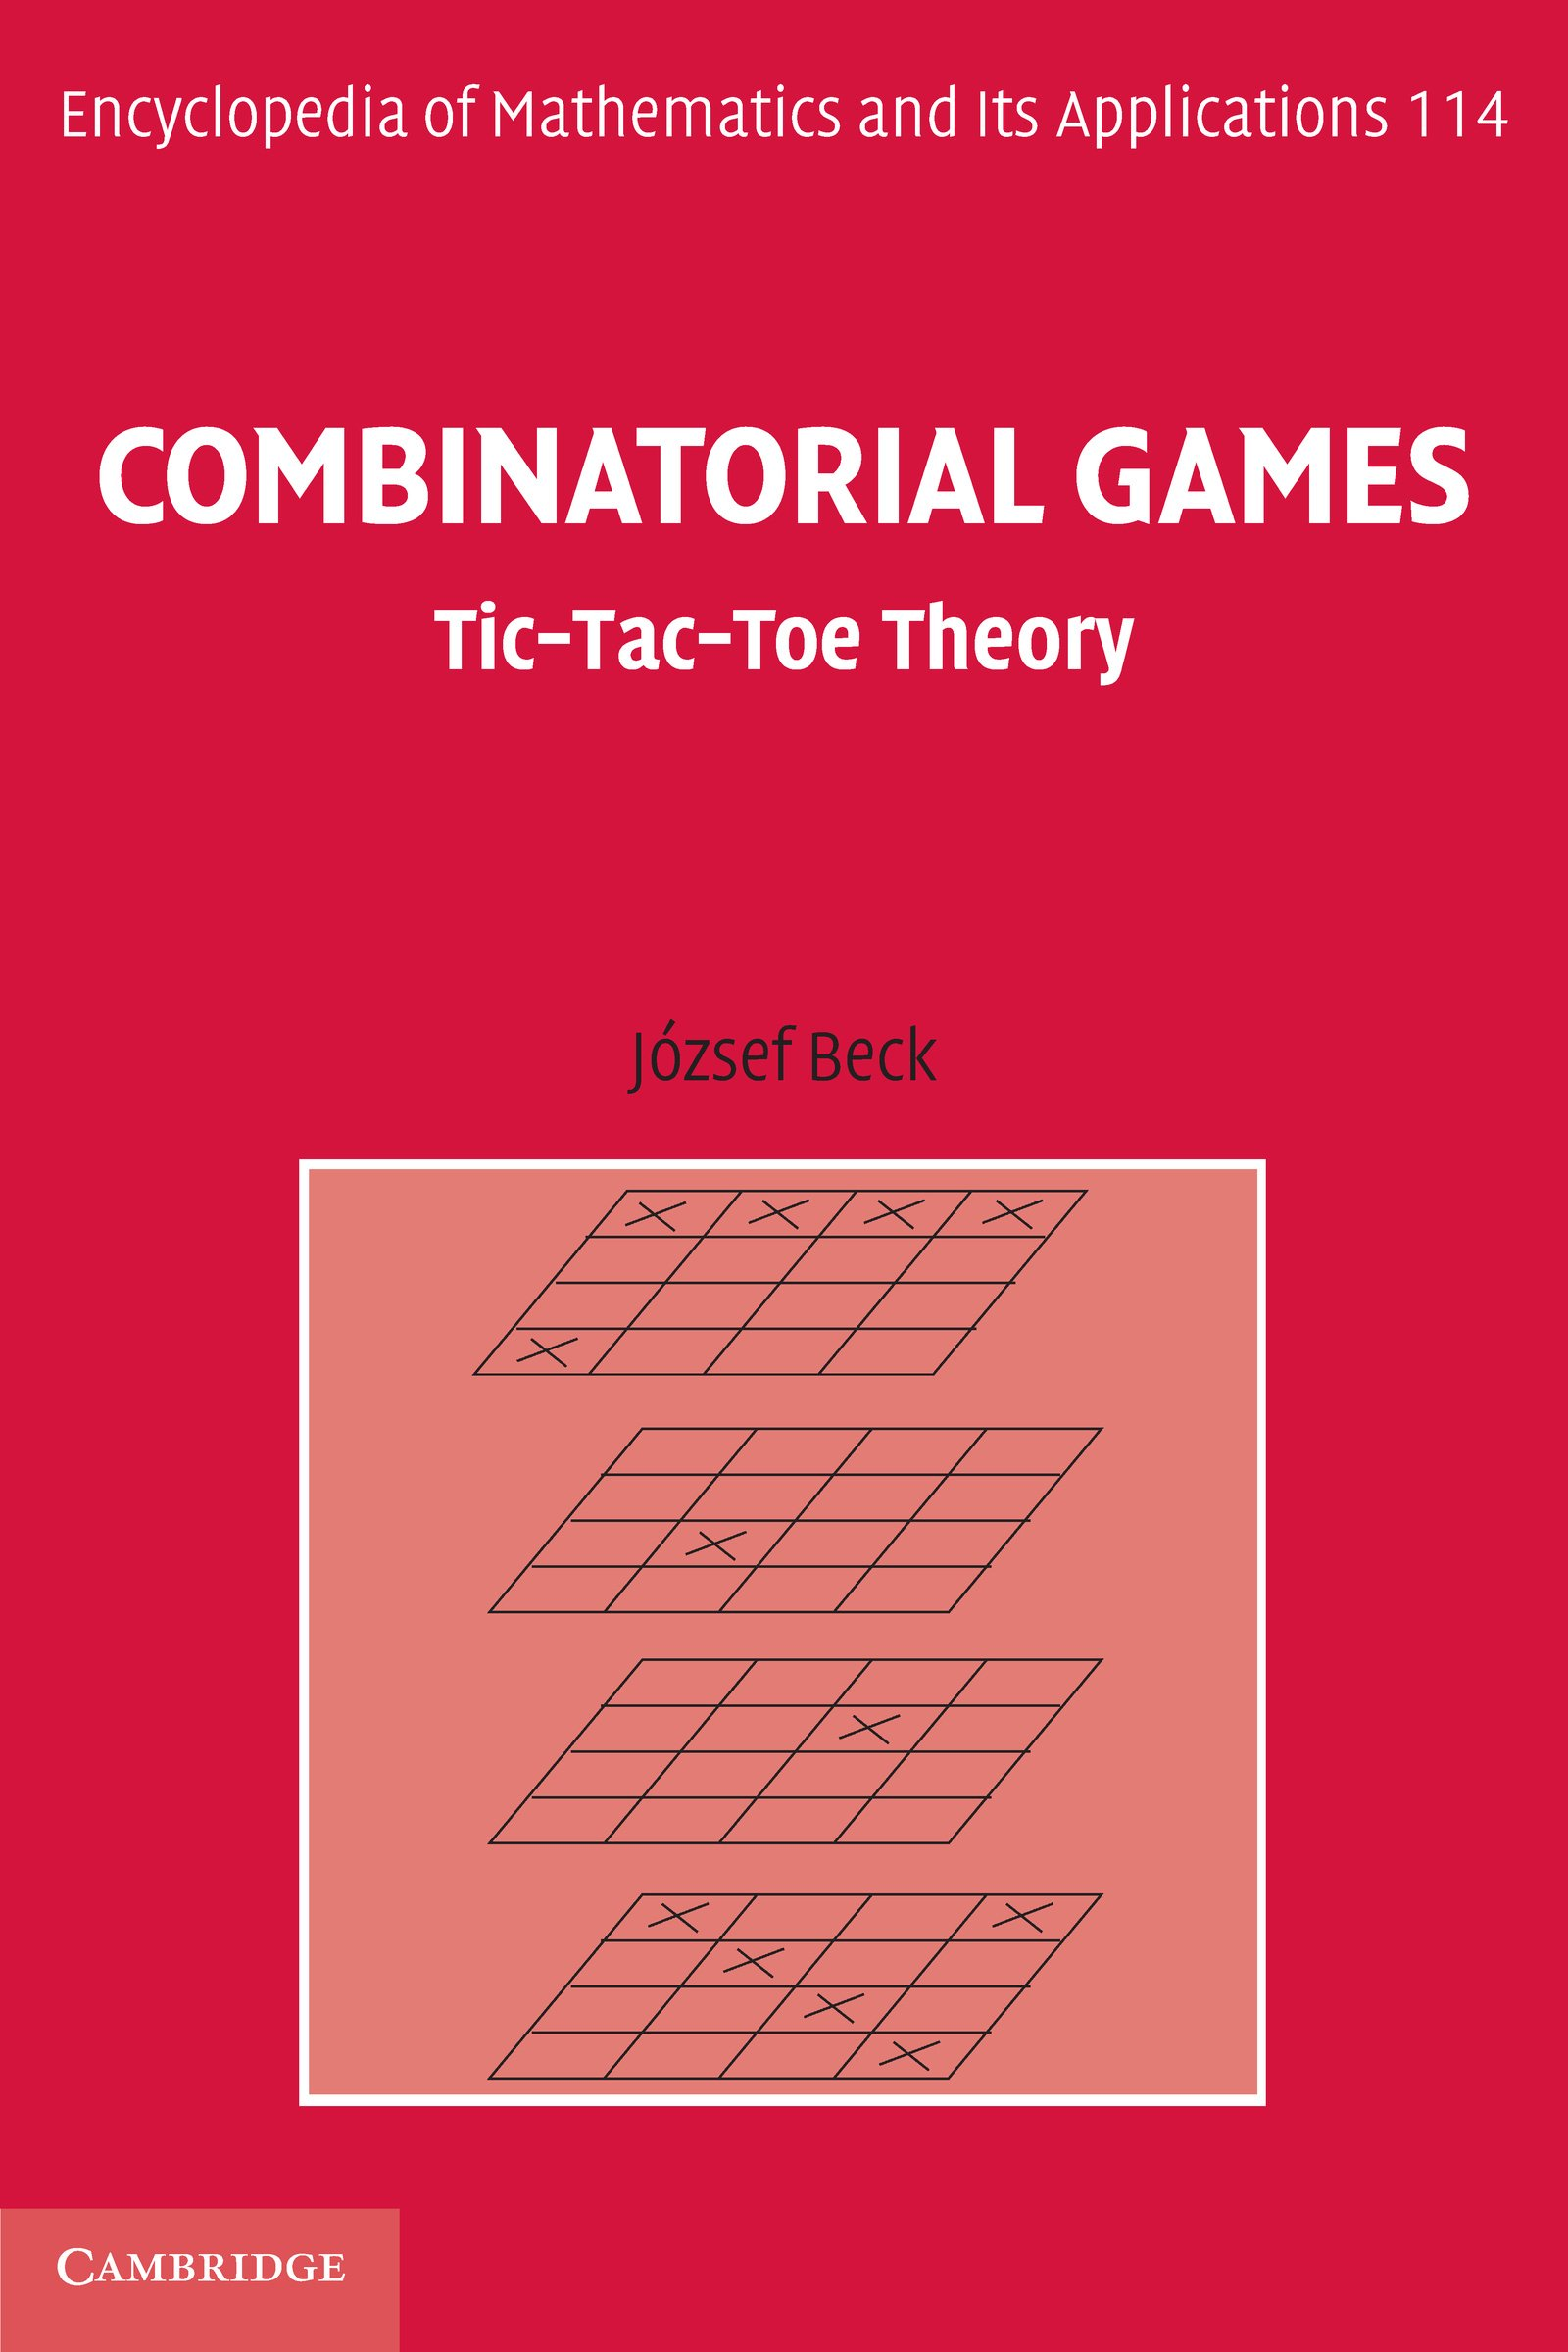
\includegraphics[width=.25\textwidth]{figures/Beck}
\pause		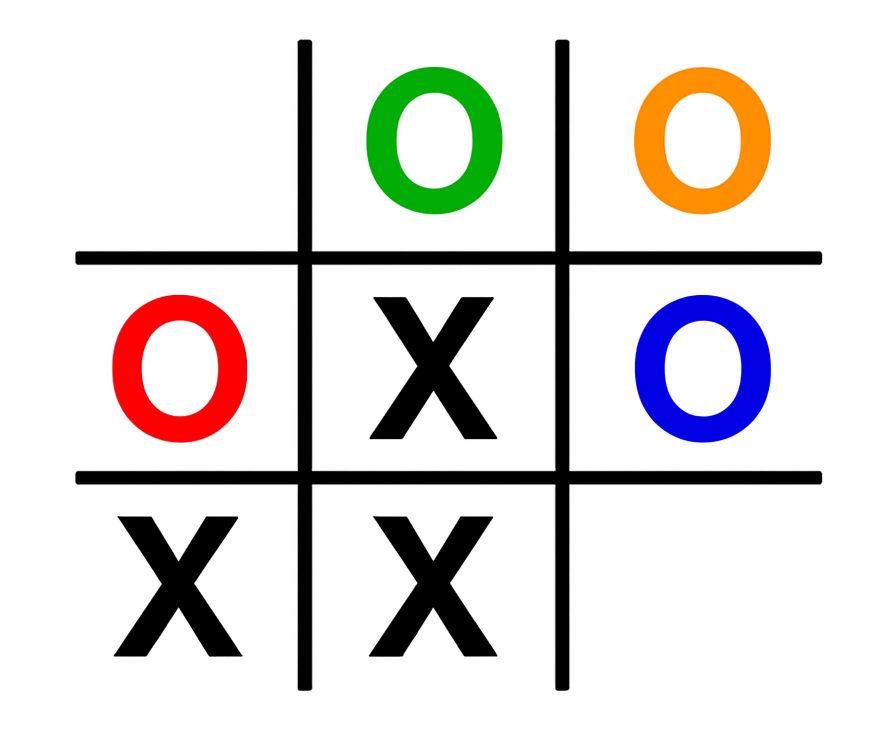
\includegraphics[width=.3\textwidth]{figures/play.png}
\end{figure}
    
\end{frame}


\begin{frame}{Example: MENACE}

\begin{itemize}
	\item Machine Educable Noughts And Crosses Engine (MENACE)
  \item Build by Donald Michie in 1961 using 304 matchboxes
\end{itemize}

\begin{center}
\only<1>{

\begin{figure}
	\centering
		
\includegraphics[width=.50\textwidth]{figures/menace_1.png}
\end{figure}
}
\only<2>{
\begin{figure}
	\centering
		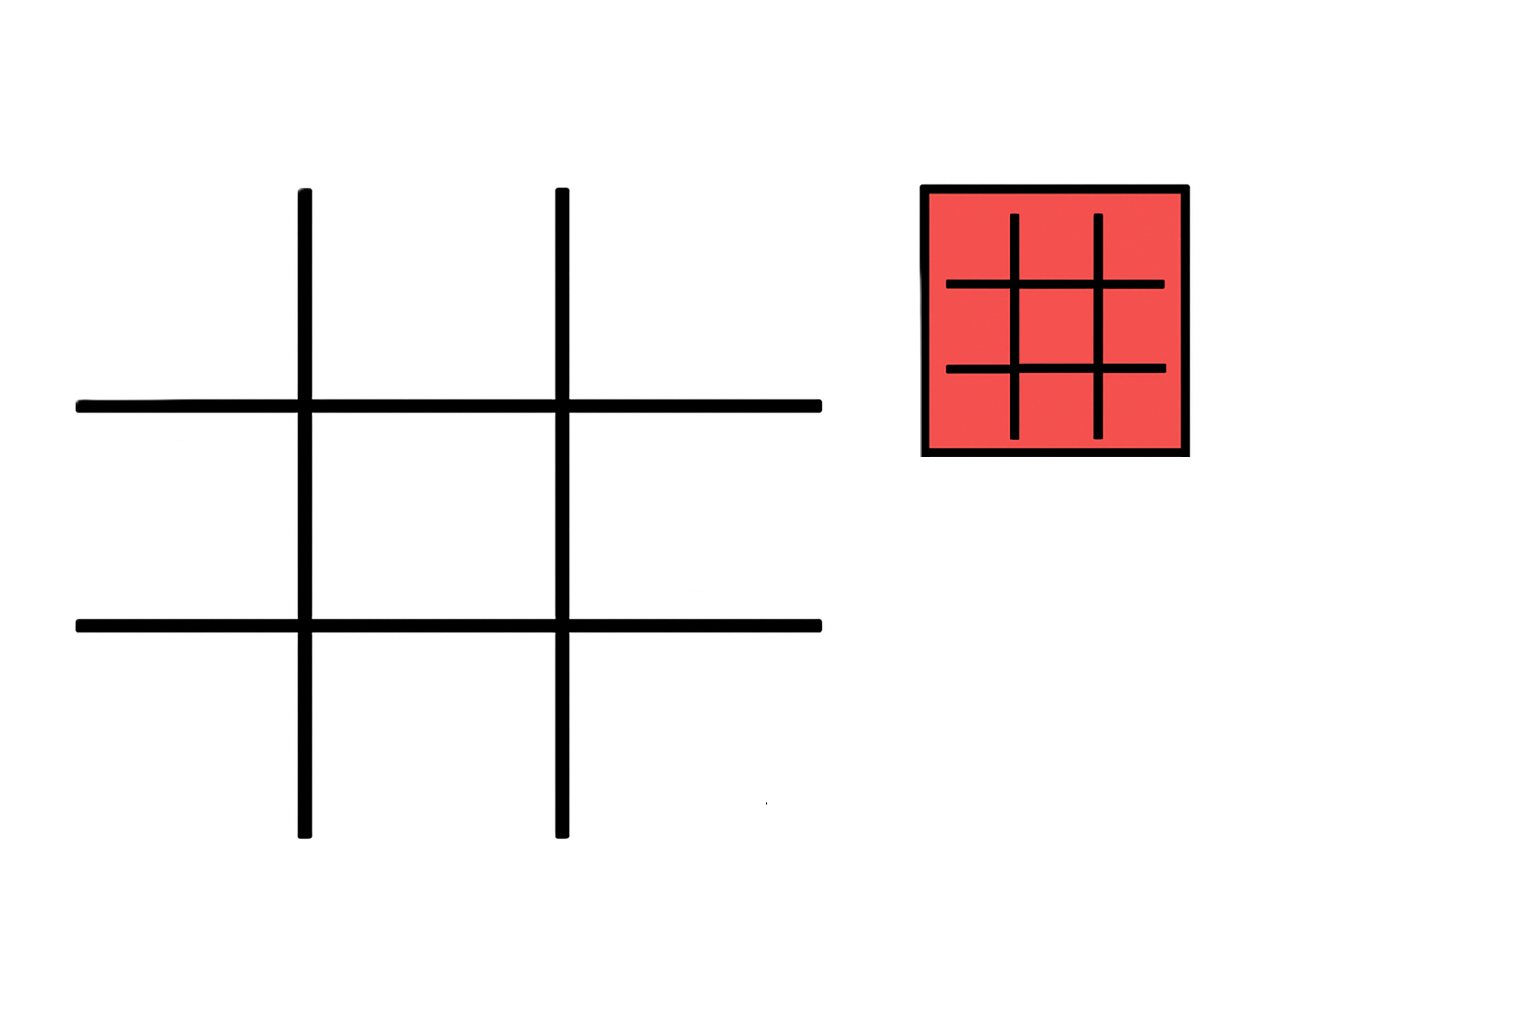
\includegraphics[width=.50\textwidth]{figures/menace_2.png}
\end{figure}
	
}
\only<3>{
\begin{figure}
	\centering
		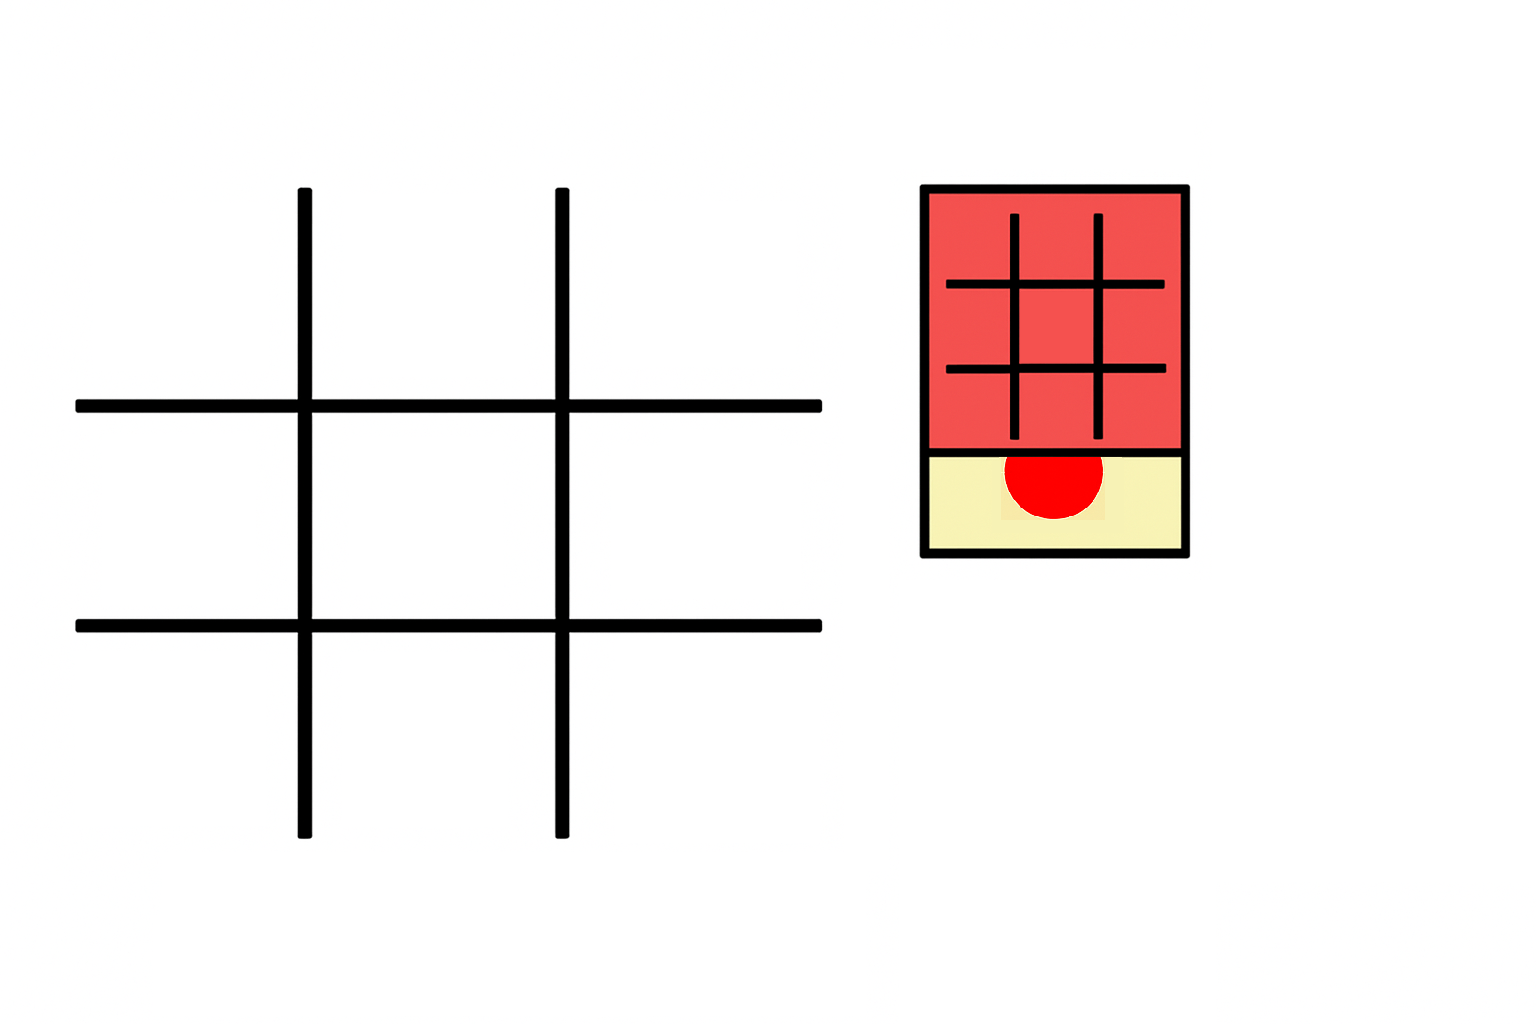
\includegraphics[width=.50\textwidth]{figures/menace_3.png}
\end{figure}
	
}
\only<4>{
\begin{figure}
	\centering
		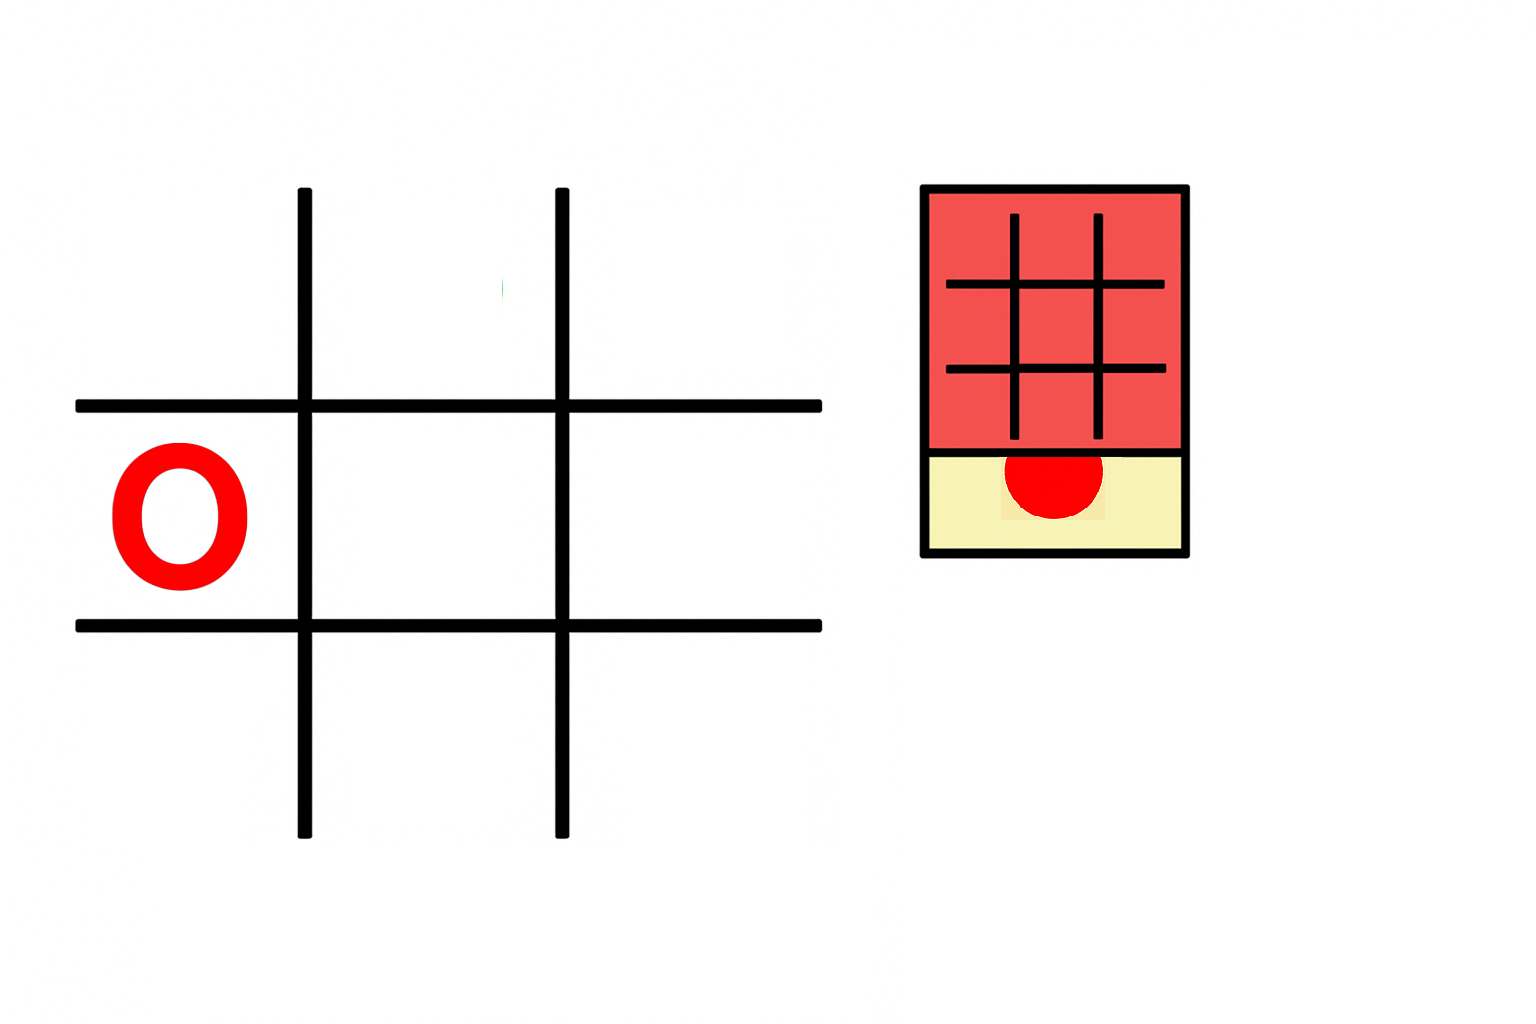
\includegraphics[width=.50\textwidth]{figures/menace_4.png}
\end{figure}
	
}
\only<5>{
\begin{figure}
	\centering
		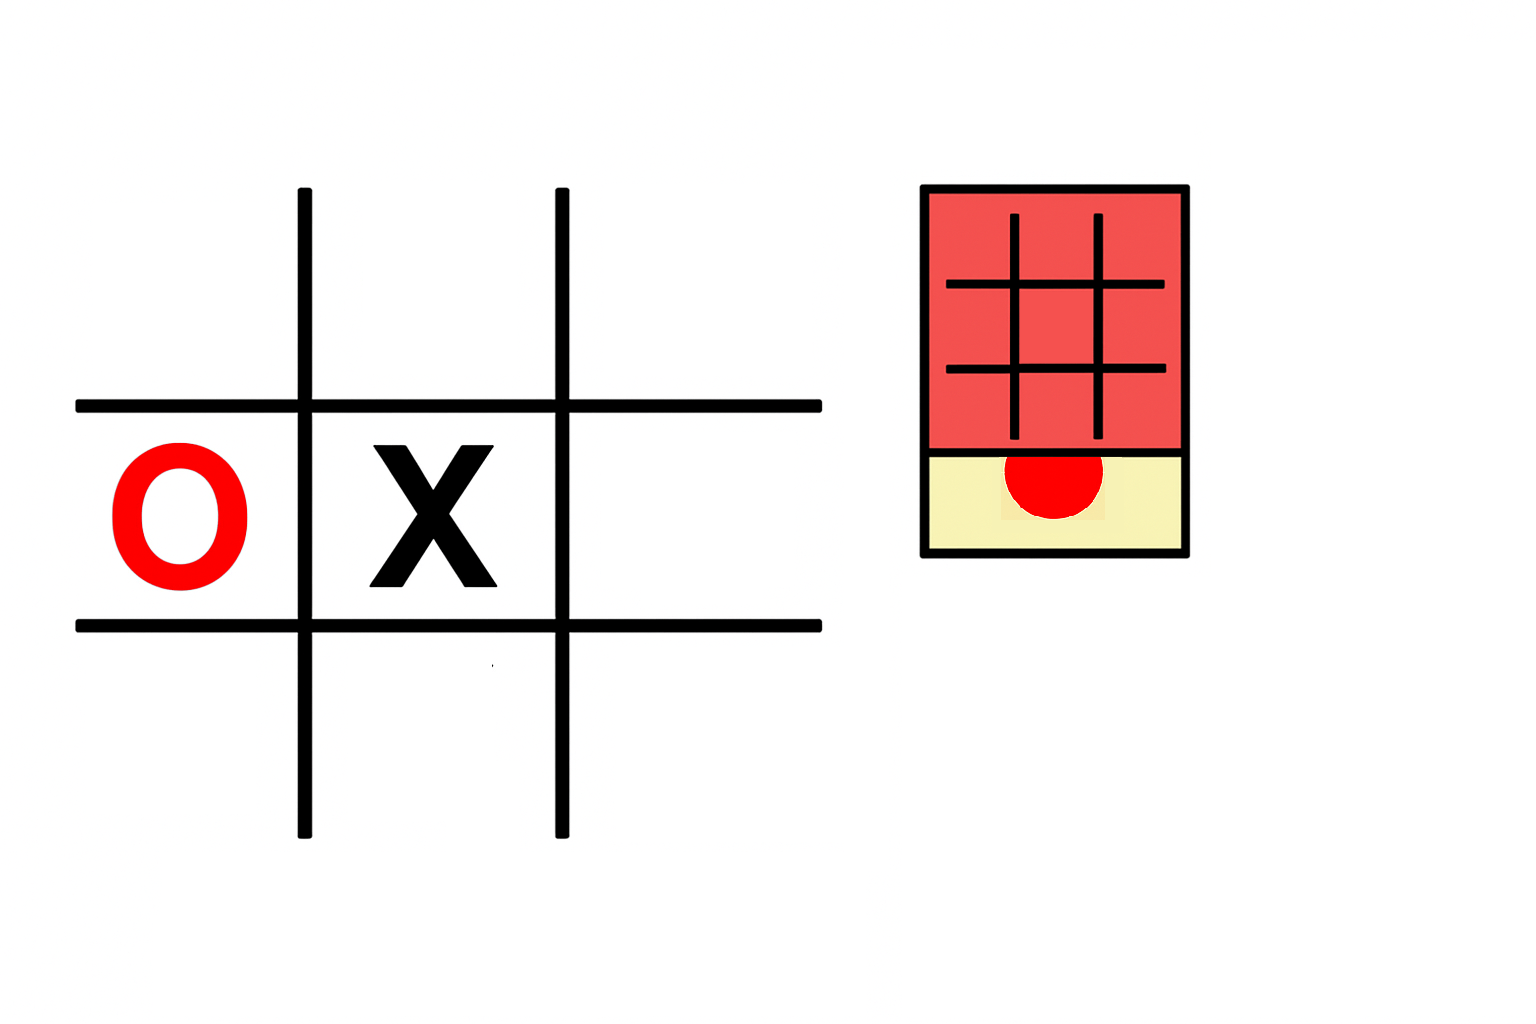
\includegraphics[width=.50\textwidth]{figures/menace_5.png}
\end{figure}
	
}
\only<6>{
\begin{figure}
	\centering
		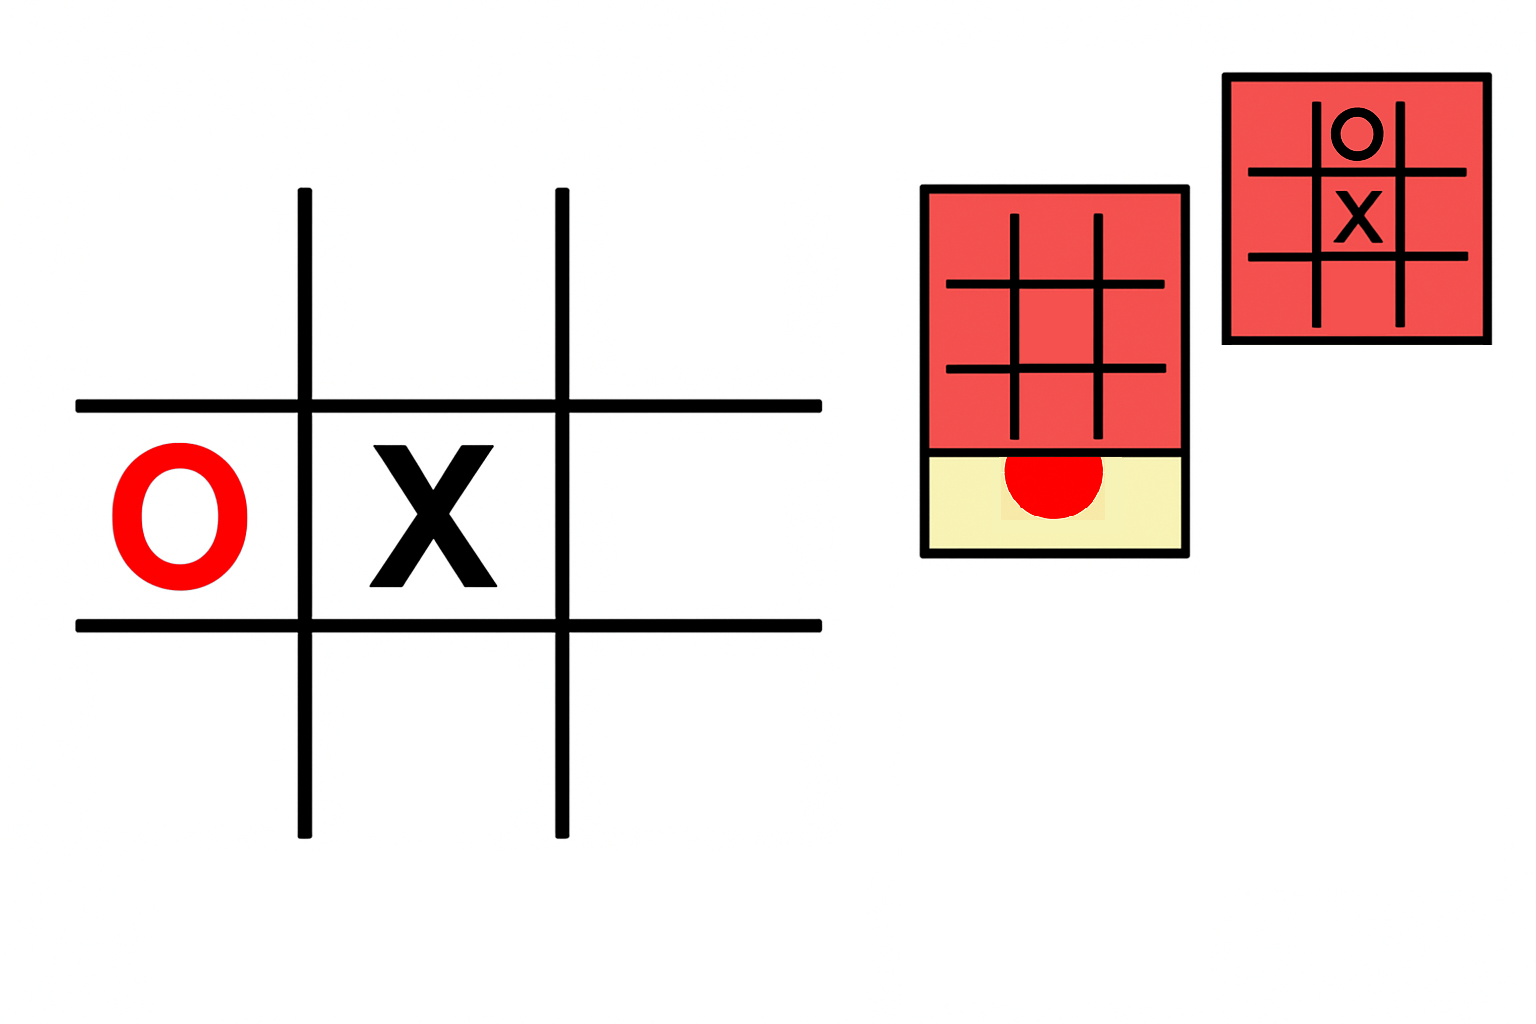
\includegraphics[width=.50\textwidth]{figures/menace_6.png}
\end{figure}
	
}
\only<7>{
\begin{figure}
	\centering
		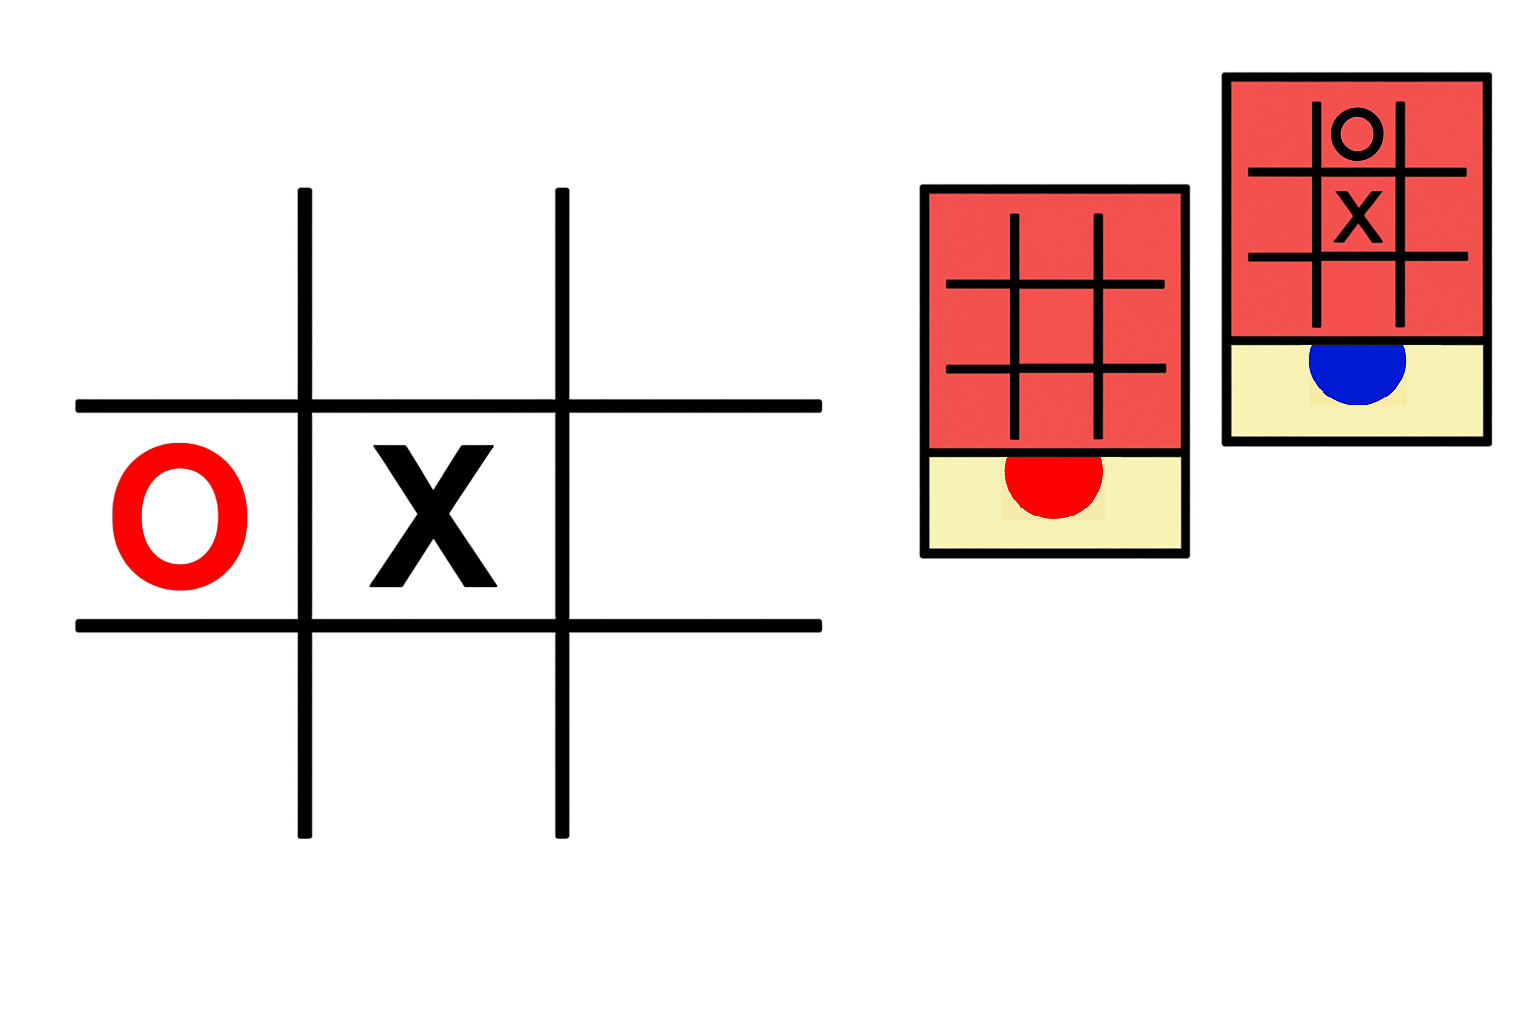
\includegraphics[width=.50\textwidth]{figures/menace_7.png}
\end{figure}
	
}
\only<8>{
\begin{figure}
	\centering
		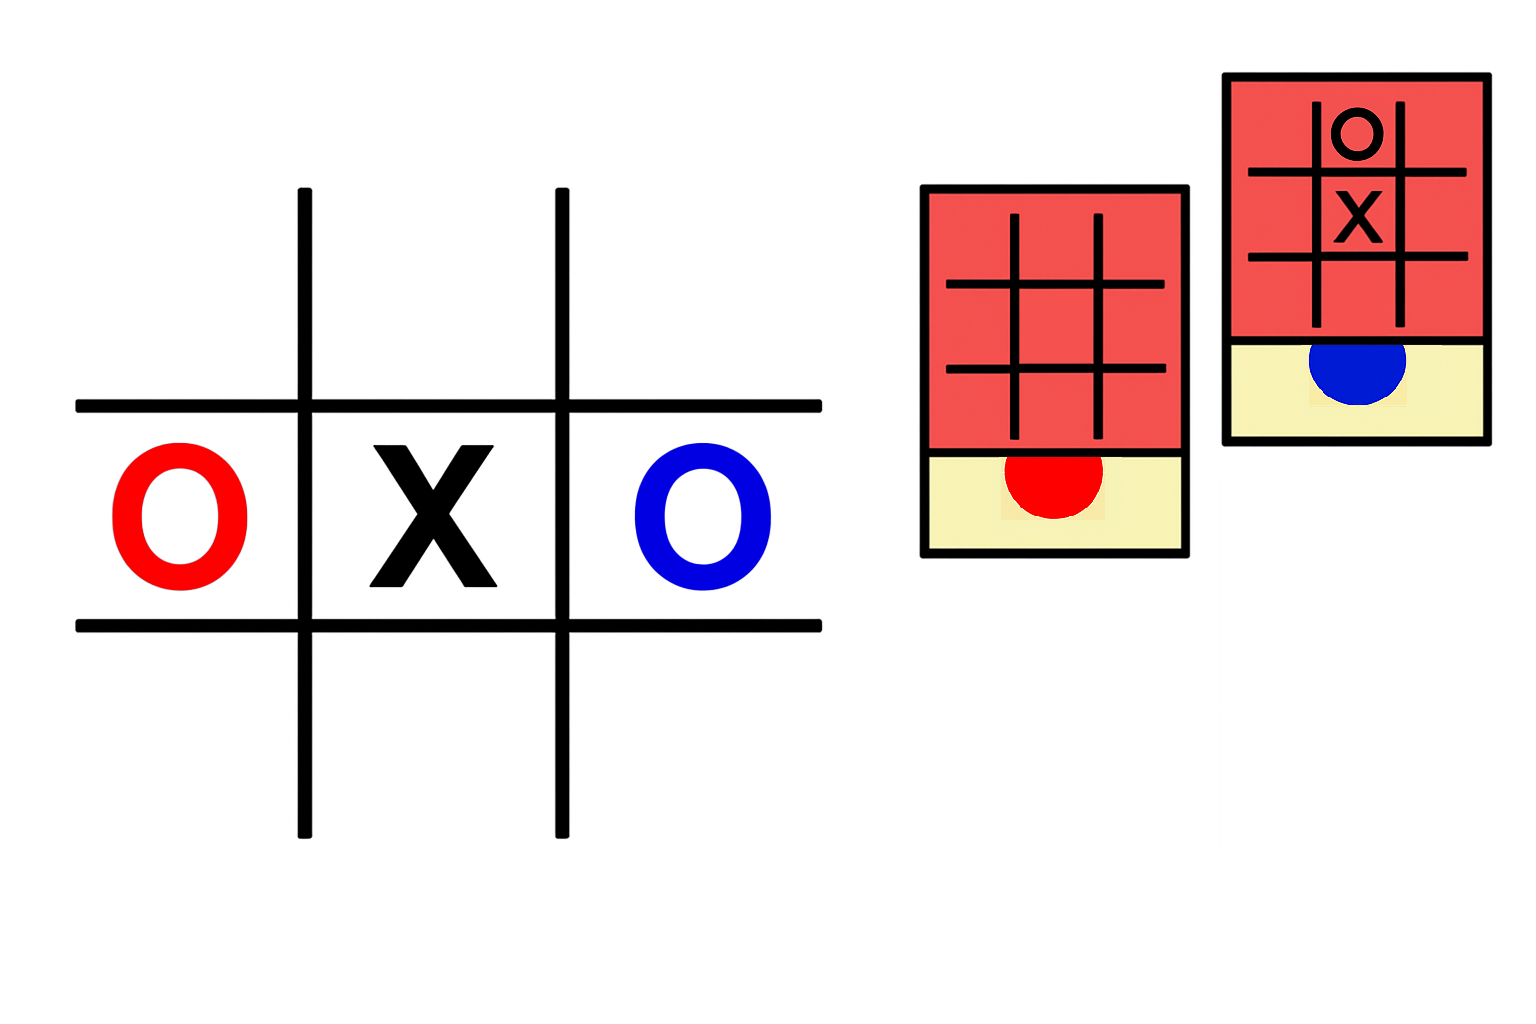
\includegraphics[width=.50\textwidth]{figures/menace_8.png}
\end{figure}
	
}
\only<9>{
\begin{figure}
    \centering
    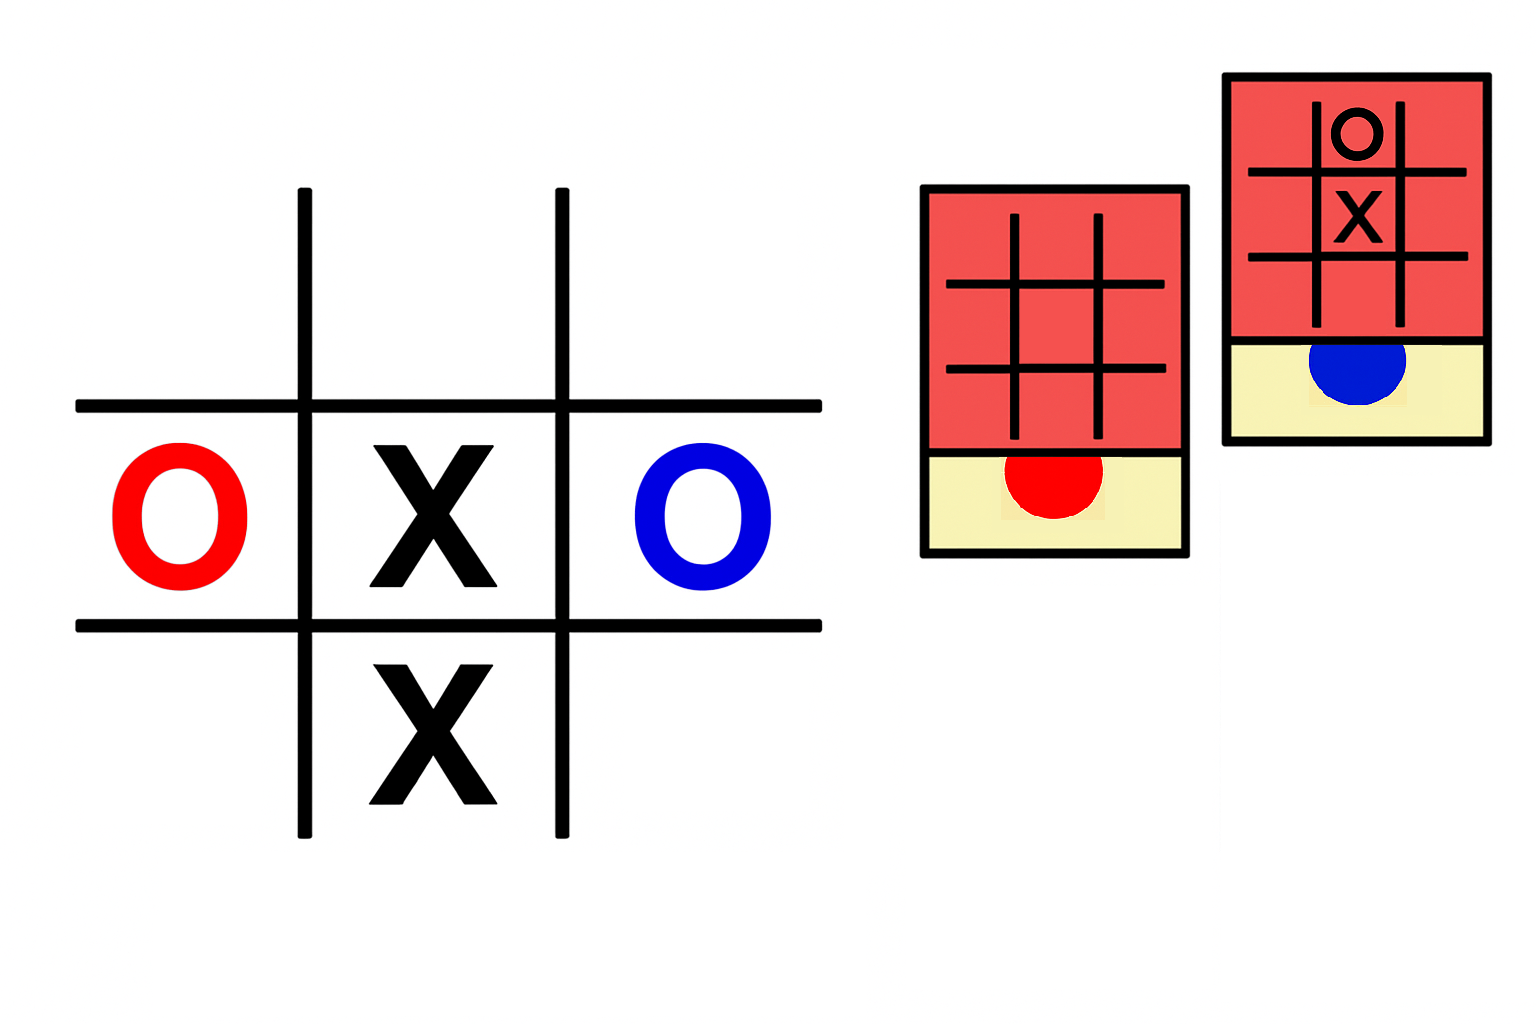
\includegraphics[width=.5\textwidth]{figures/menace_9.png}
\end{figure}
}
\only<10>{
\begin{figure}
    \centering
    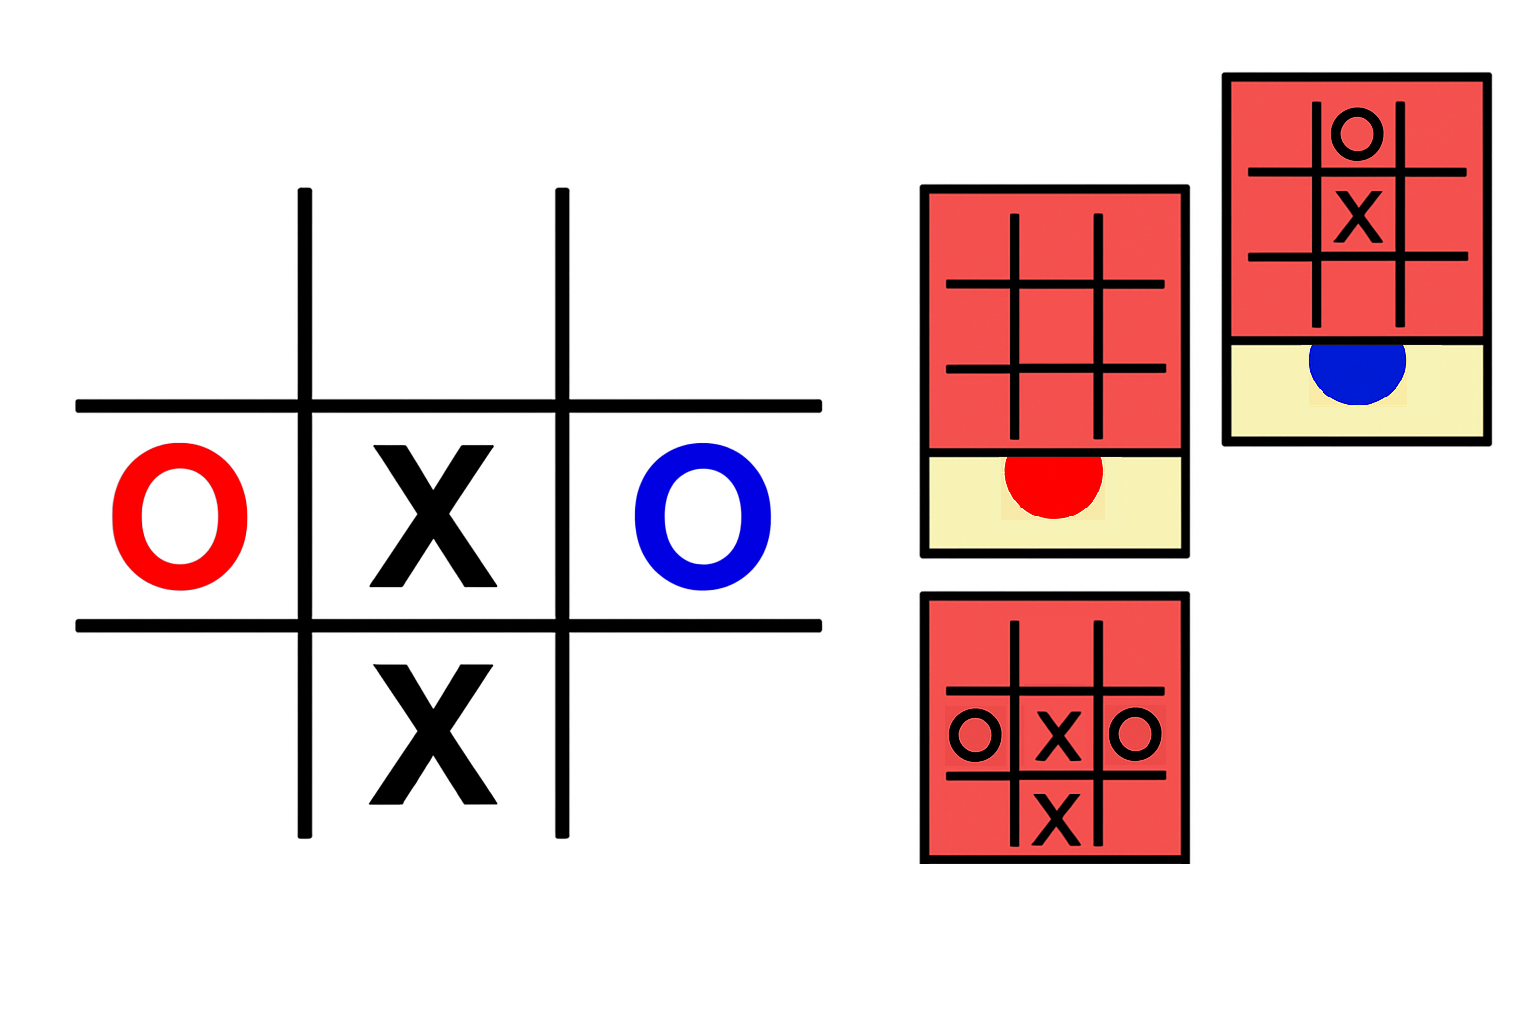
\includegraphics[width=.5\textwidth]{figures/menace_10.png}
\end{figure}
}
\only<11>{
\begin{figure}
    \centering
    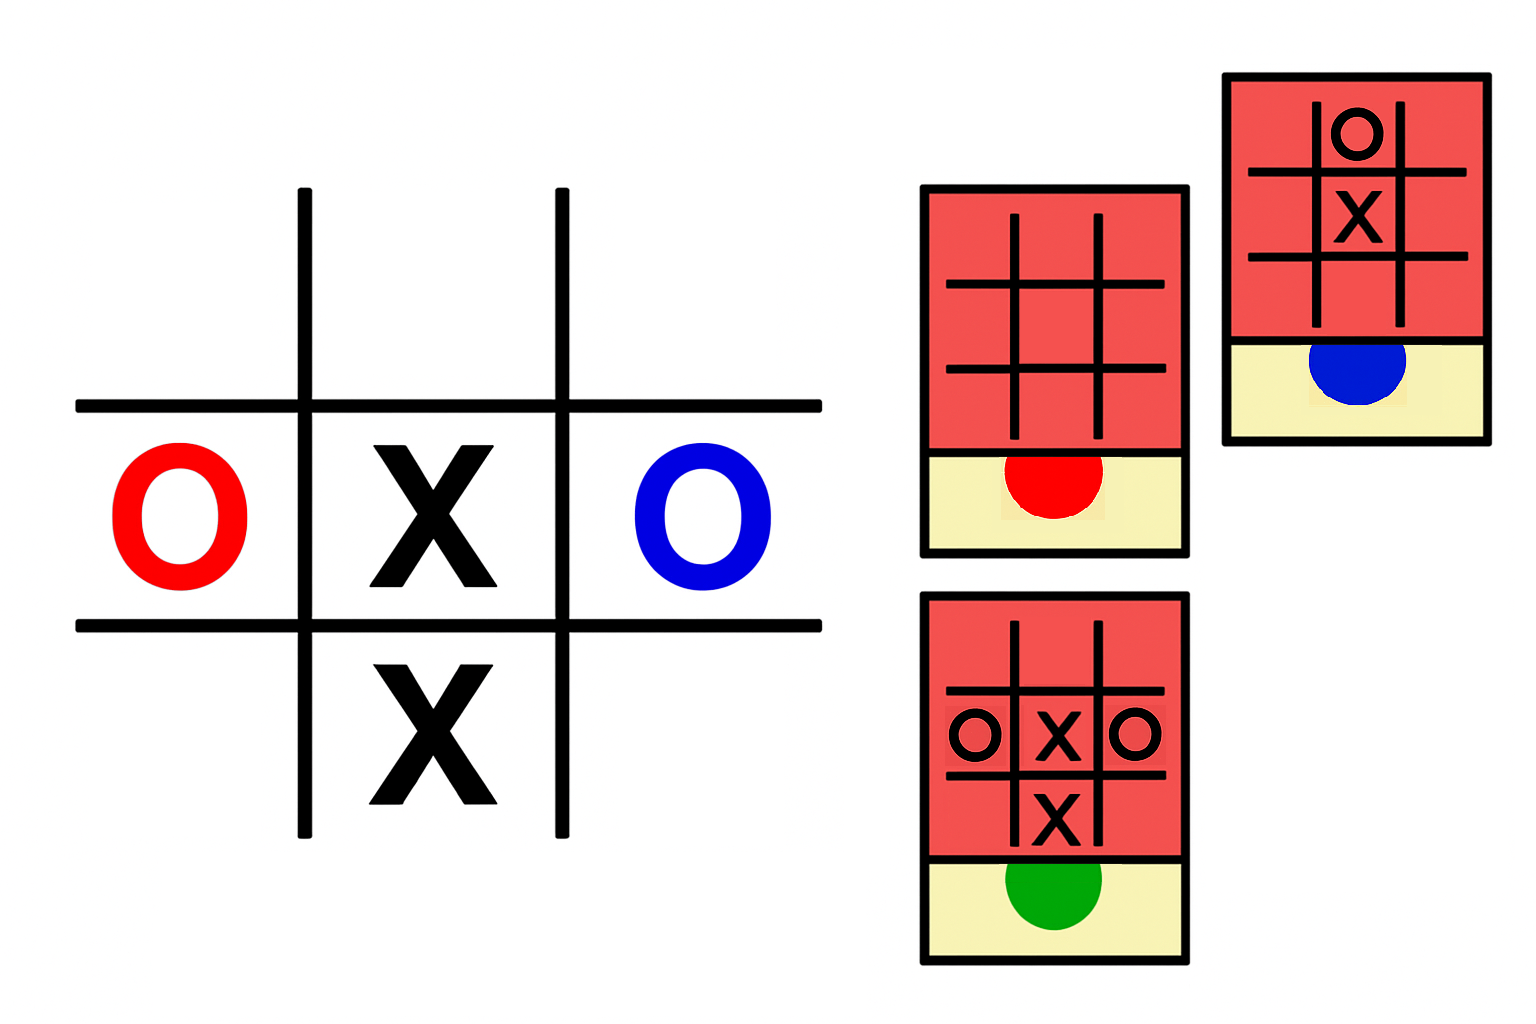
\includegraphics[width=.5\textwidth]{figures/menace_11.png}
\end{figure}
}
\only<12>{
\begin{figure}
    \centering
    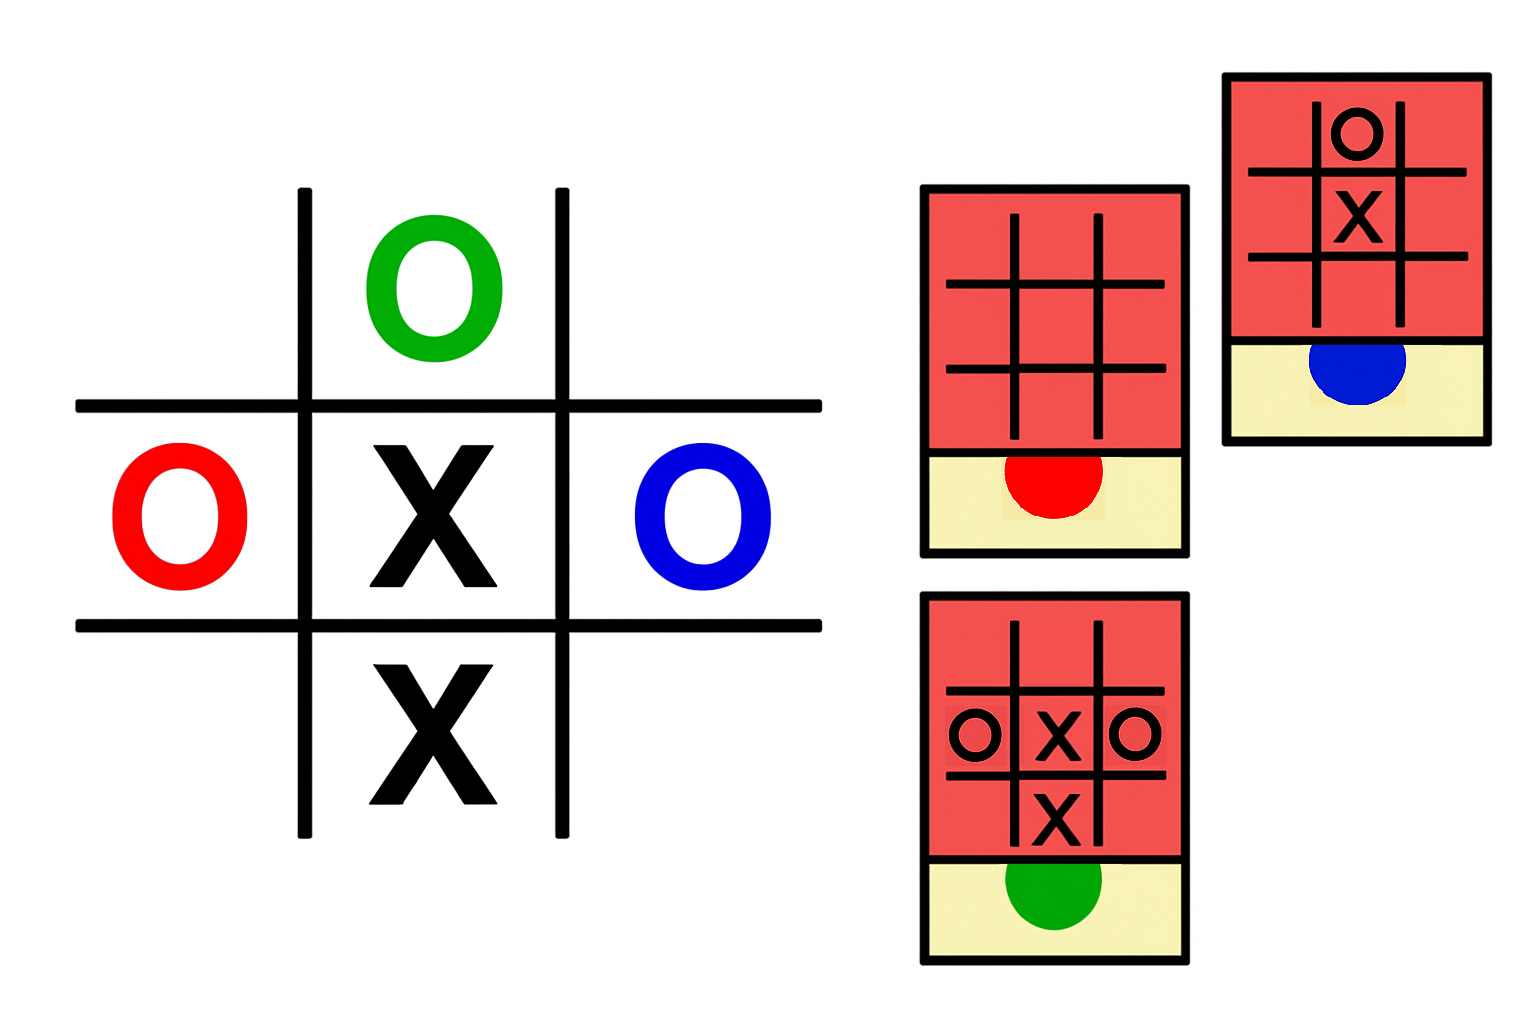
\includegraphics[width=.5\textwidth]{figures/menace_12.png}
\end{figure}
}
\only<13>{
\begin{figure}
    \centering
    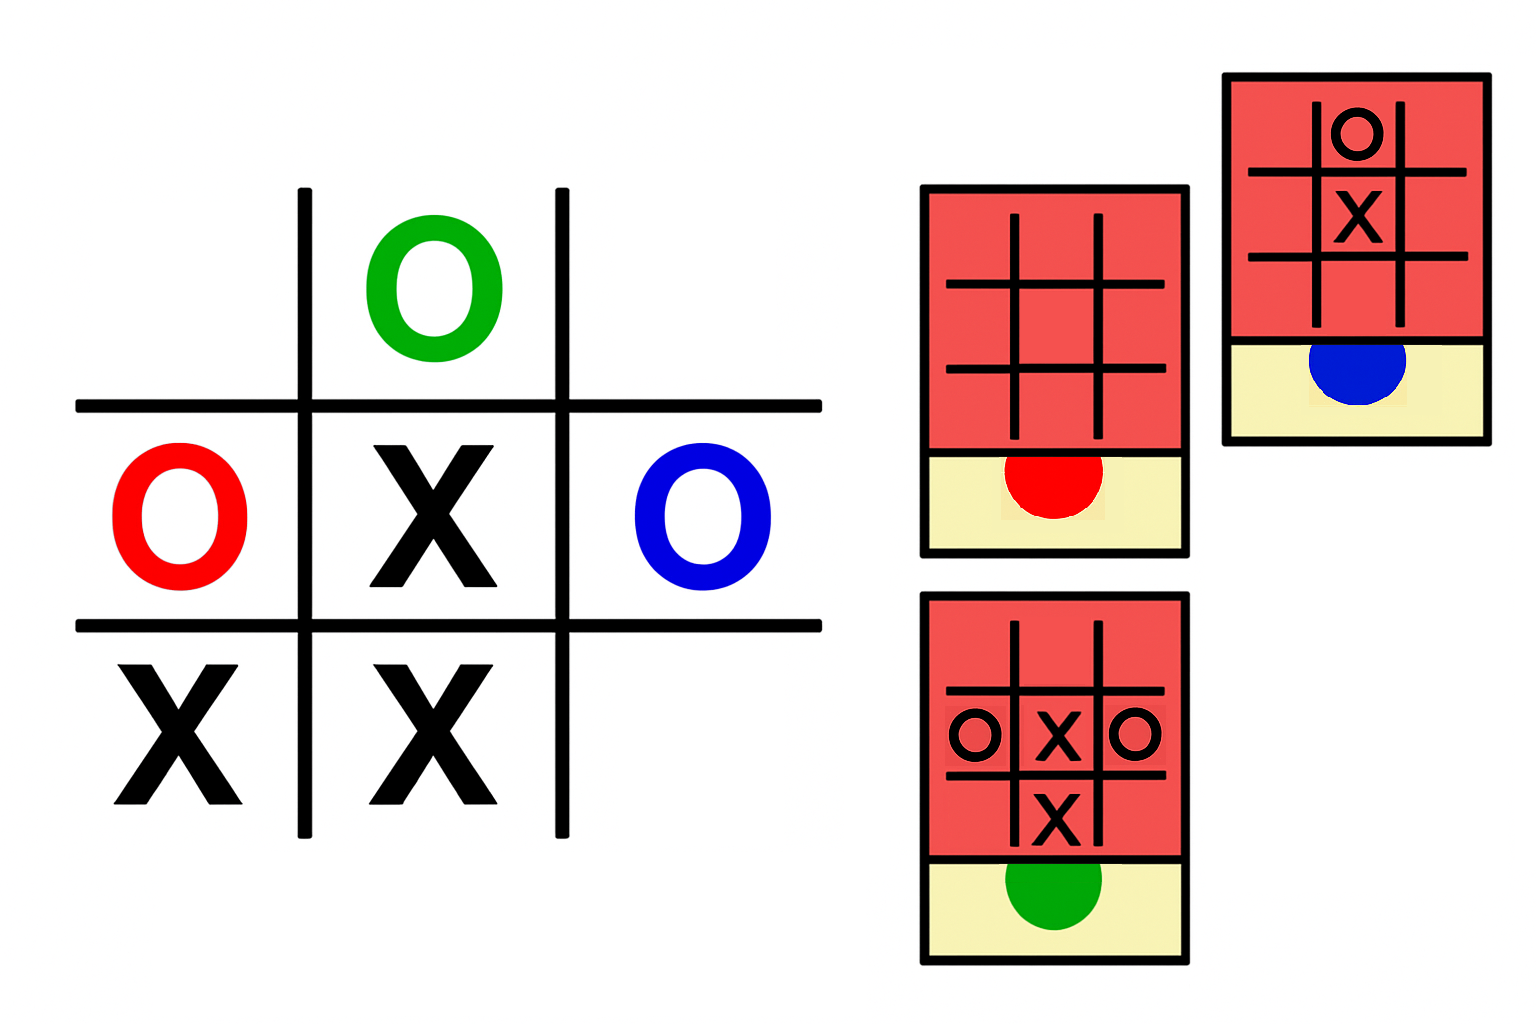
\includegraphics[width=.5\textwidth]{figures/menace_13.png}
\end{figure}
}
\only<14>{
\begin{figure}
    \centering
    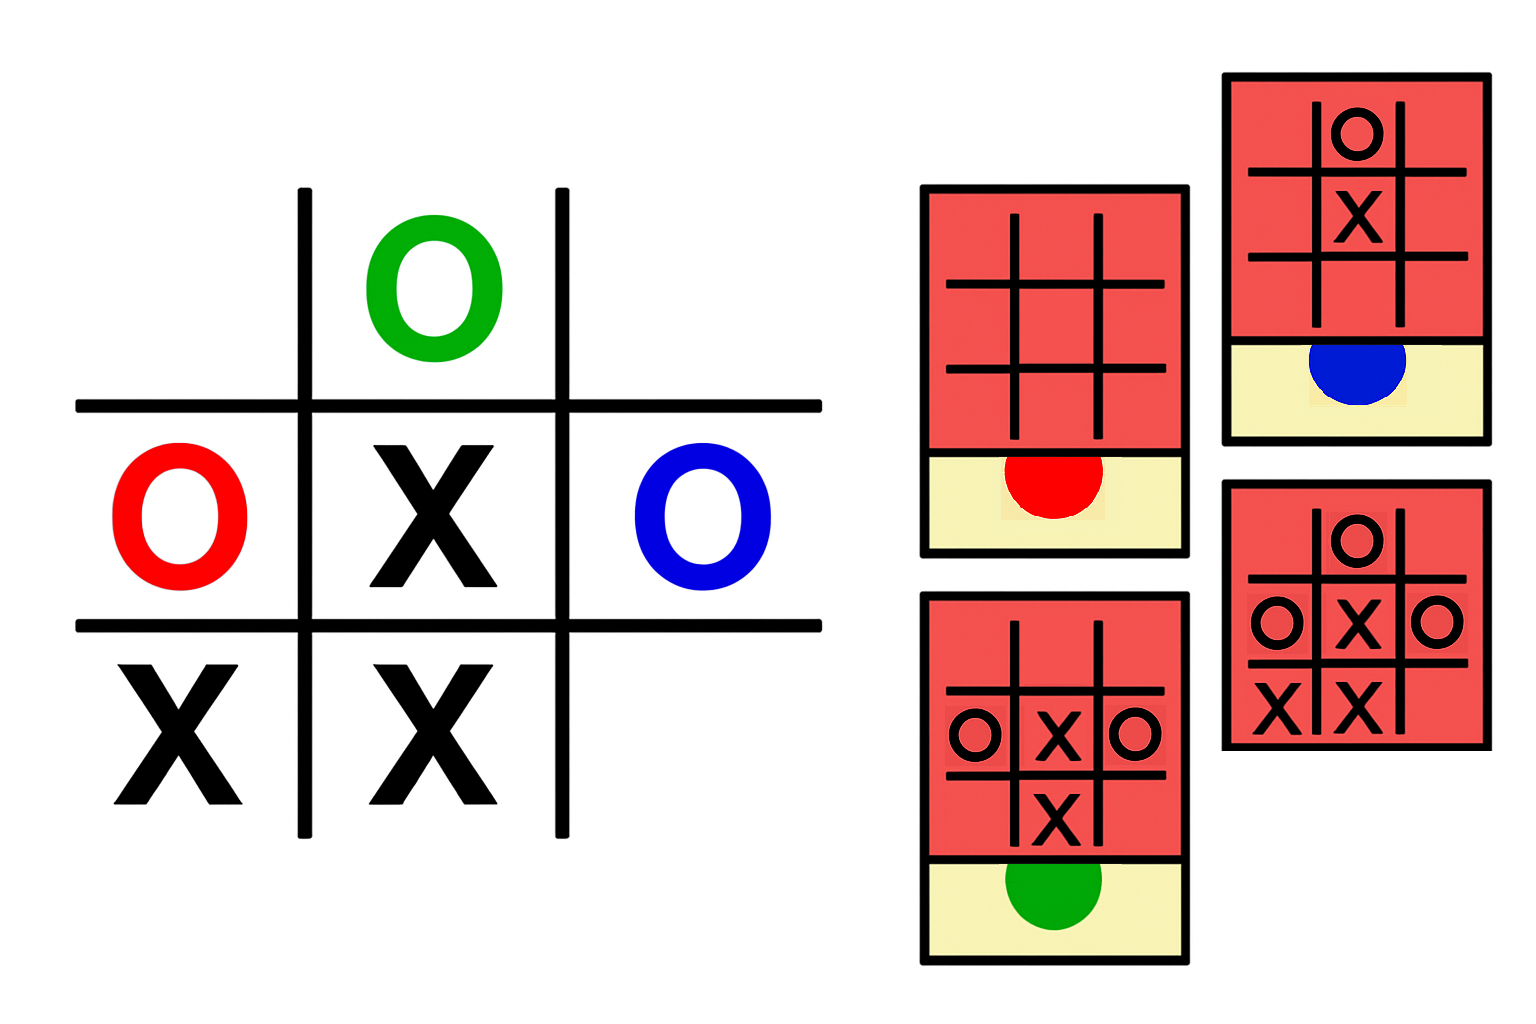
\includegraphics[width=.5\textwidth]{figures/menace_14.png}
\end{figure}
}
\only<15>{
\begin{figure}
    \centering
    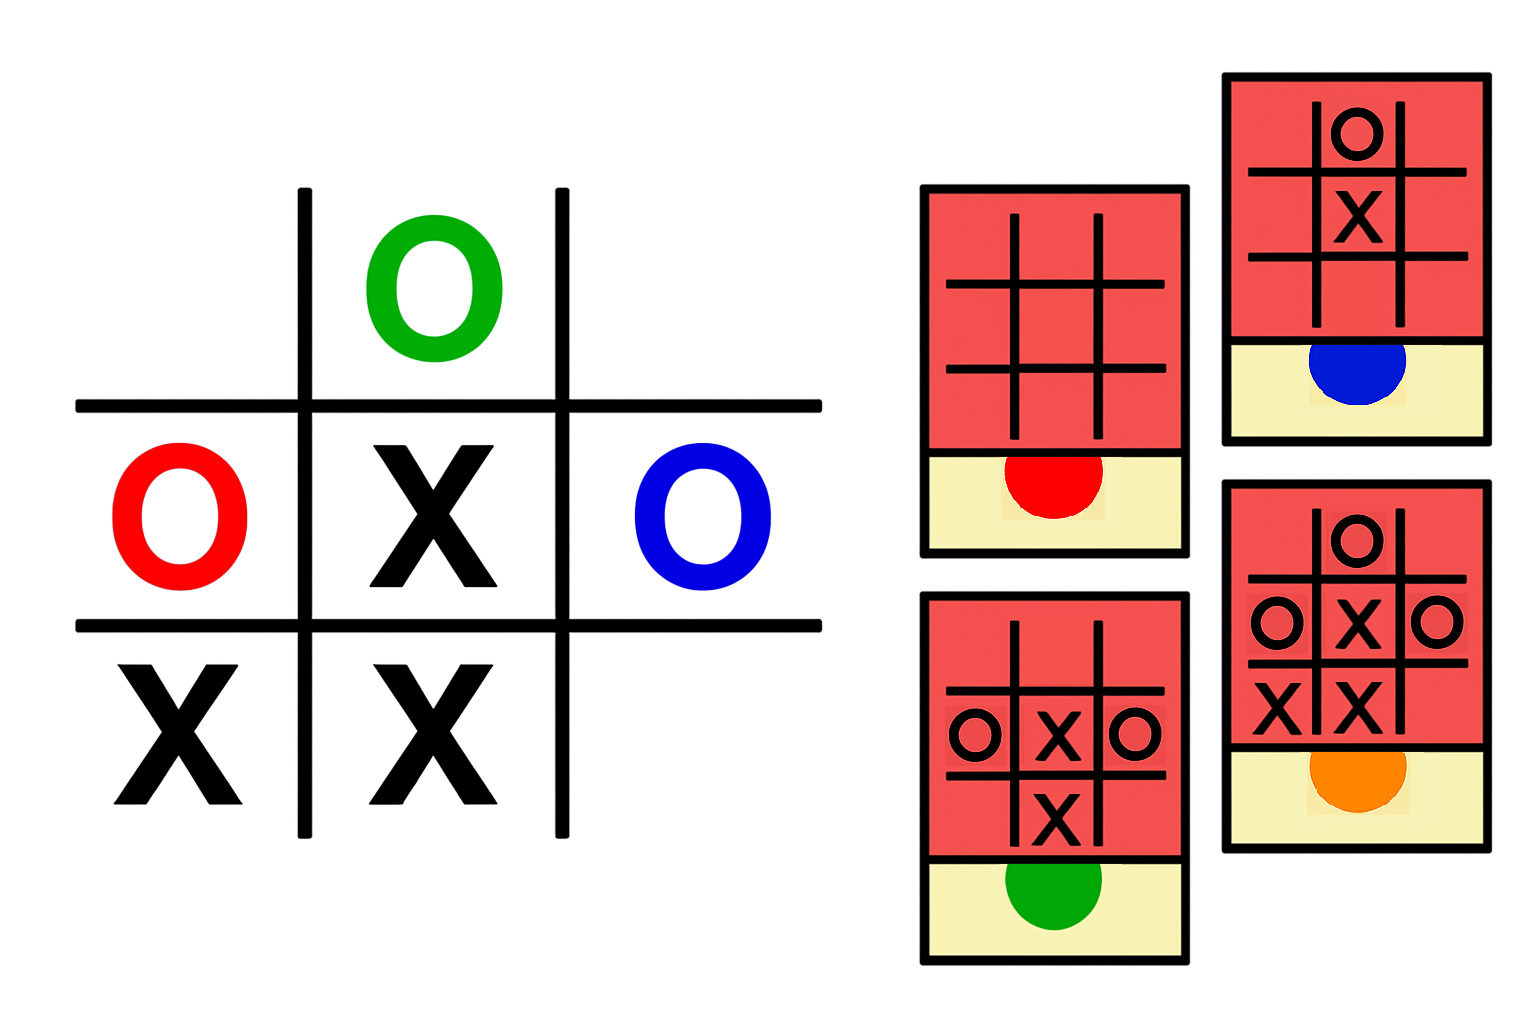
\includegraphics[width=.5\textwidth]{figures/menace_15.png}
\end{figure}
}
\only<16>{
\begin{figure}
    \centering
    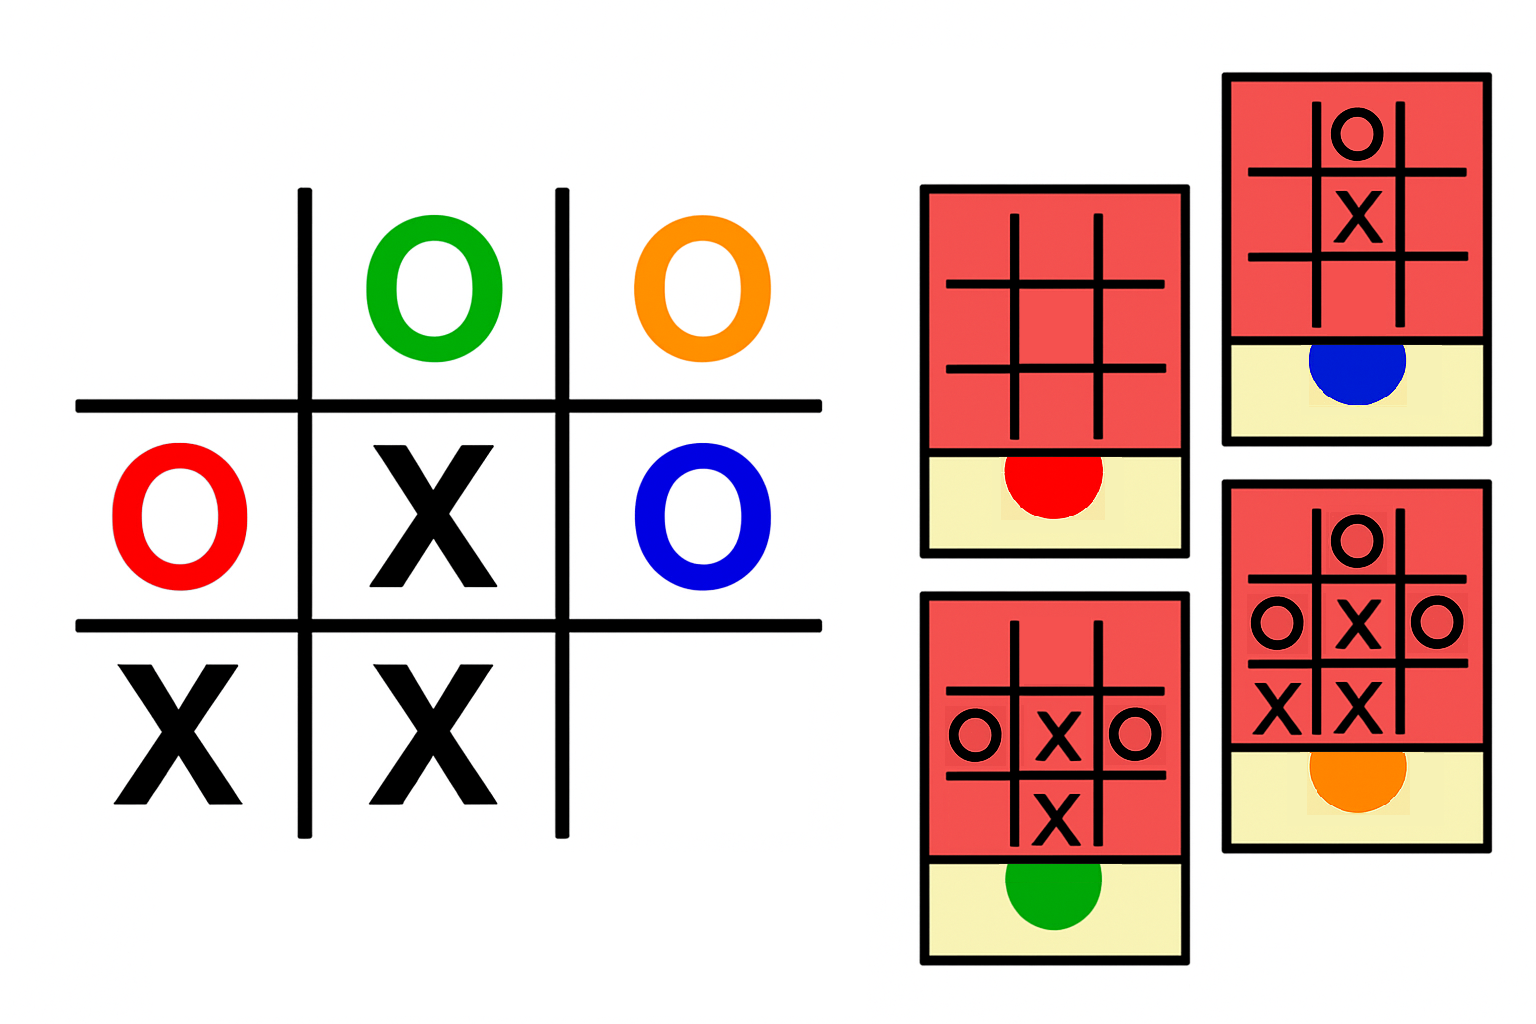
\includegraphics[width=.5\textwidth]{figures/menace_16.png}
\end{figure}
}
\only<17>{
\begin{figure}
    \centering
    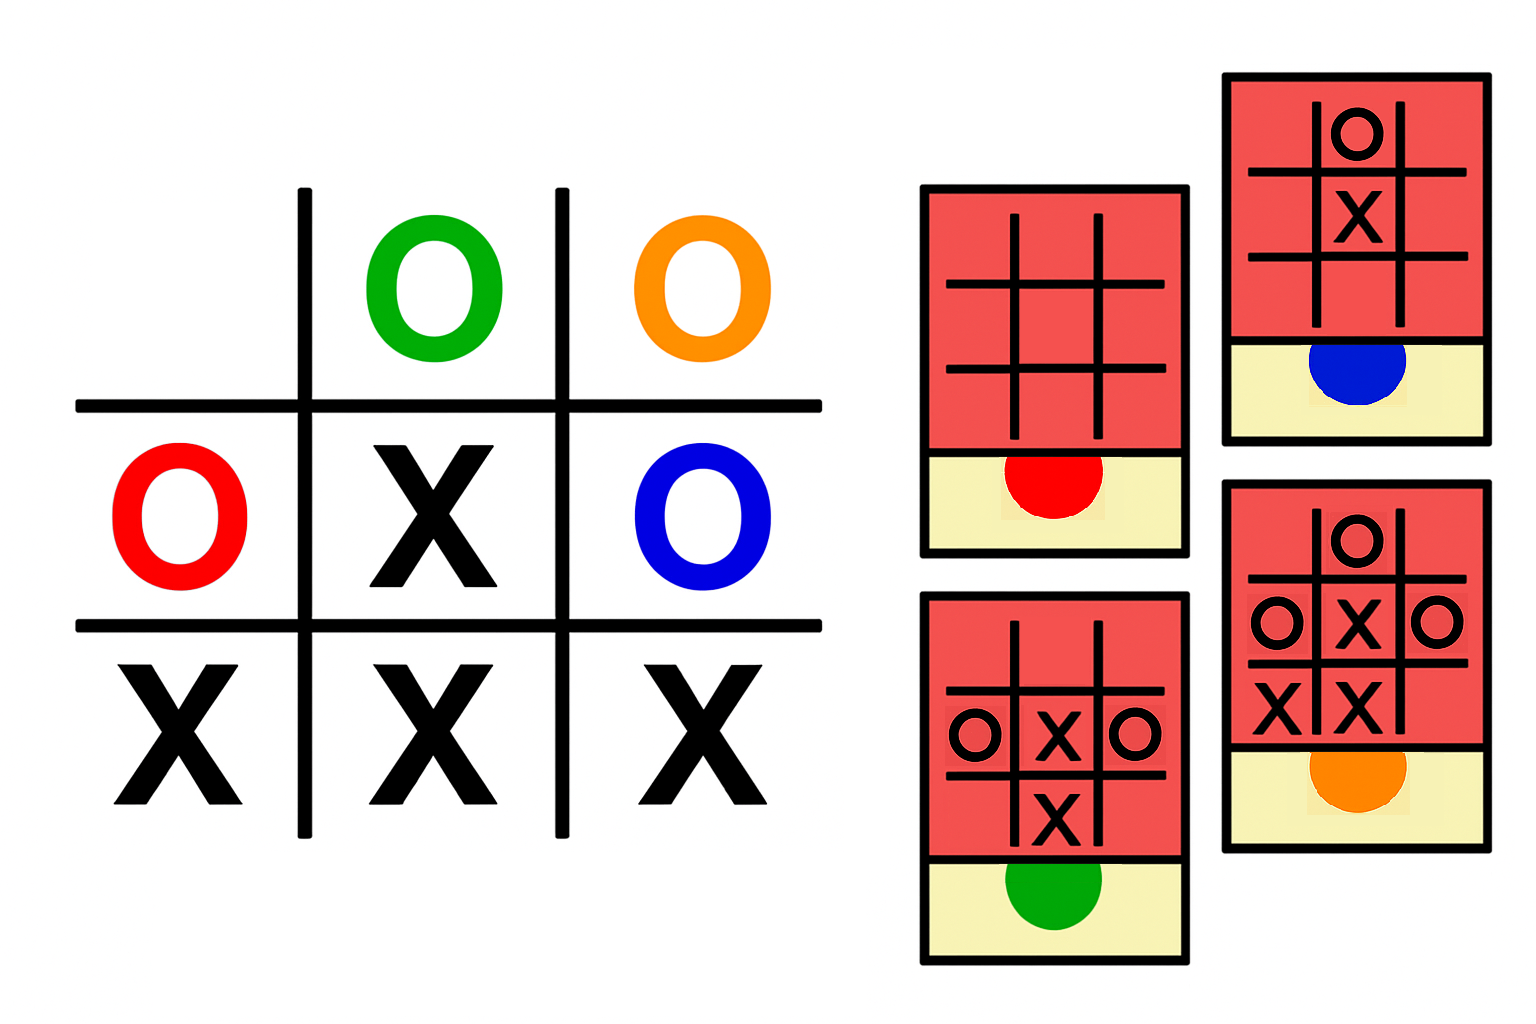
\includegraphics[width=.5\textwidth]{figures/menace_17.png}
\end{figure}
}
\only<18>{
\begin{figure}
    \centering
    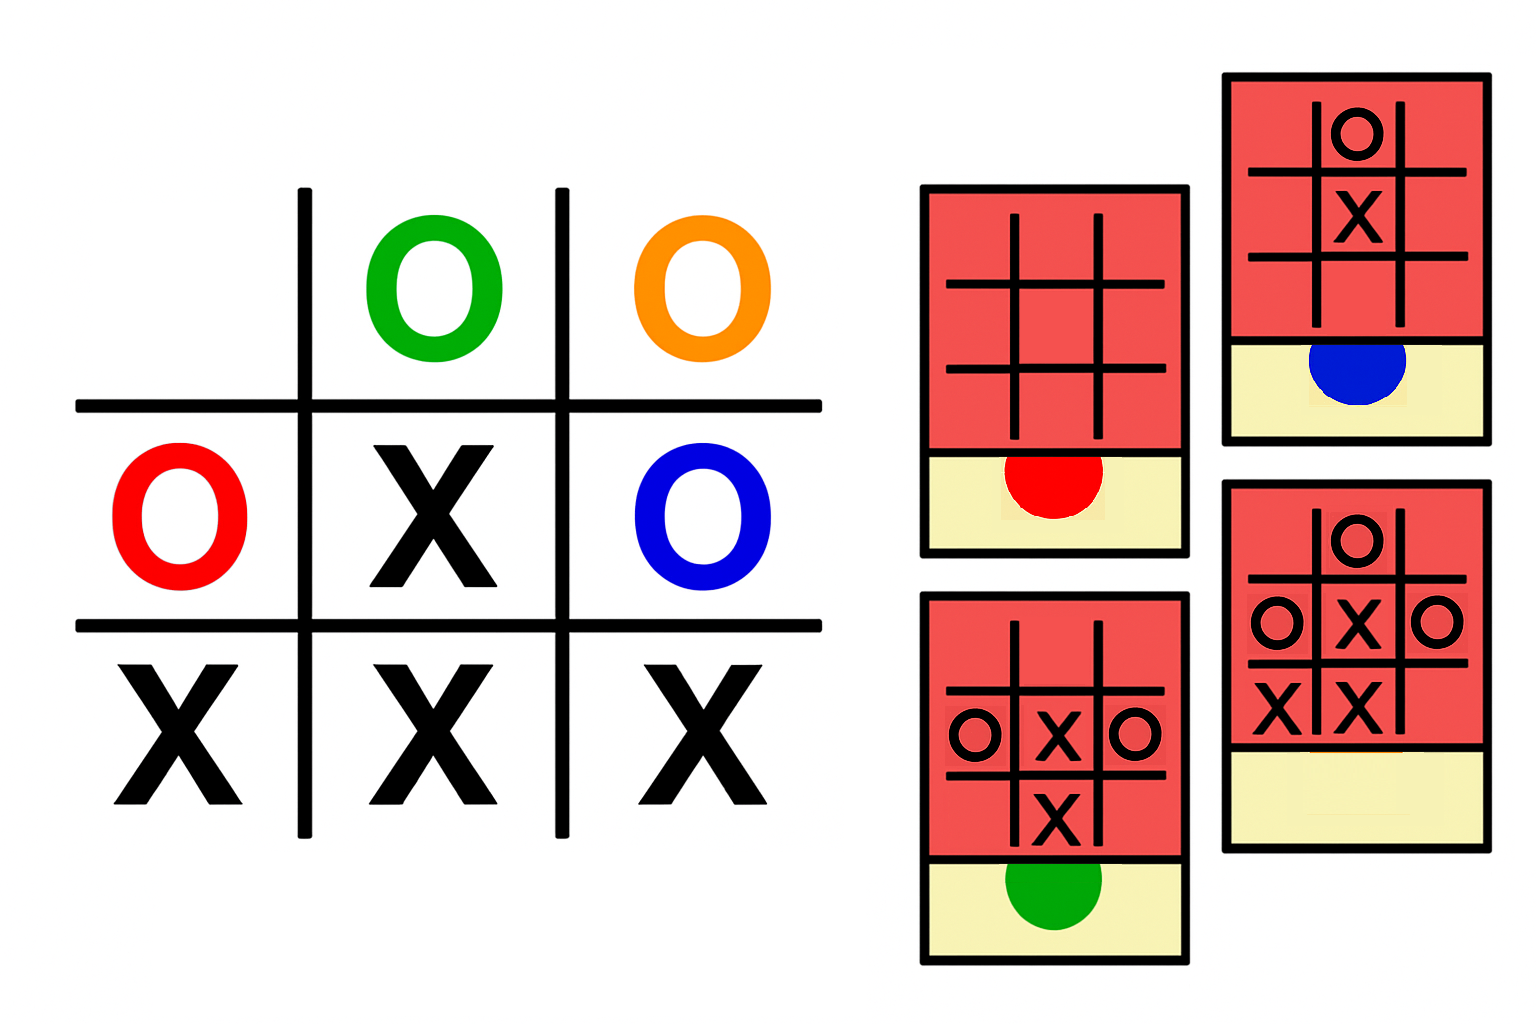
\includegraphics[width=.5\textwidth]{figures/menace_18.png}
\end{figure}
}
\only<19>{
\begin{figure}
    \centering
    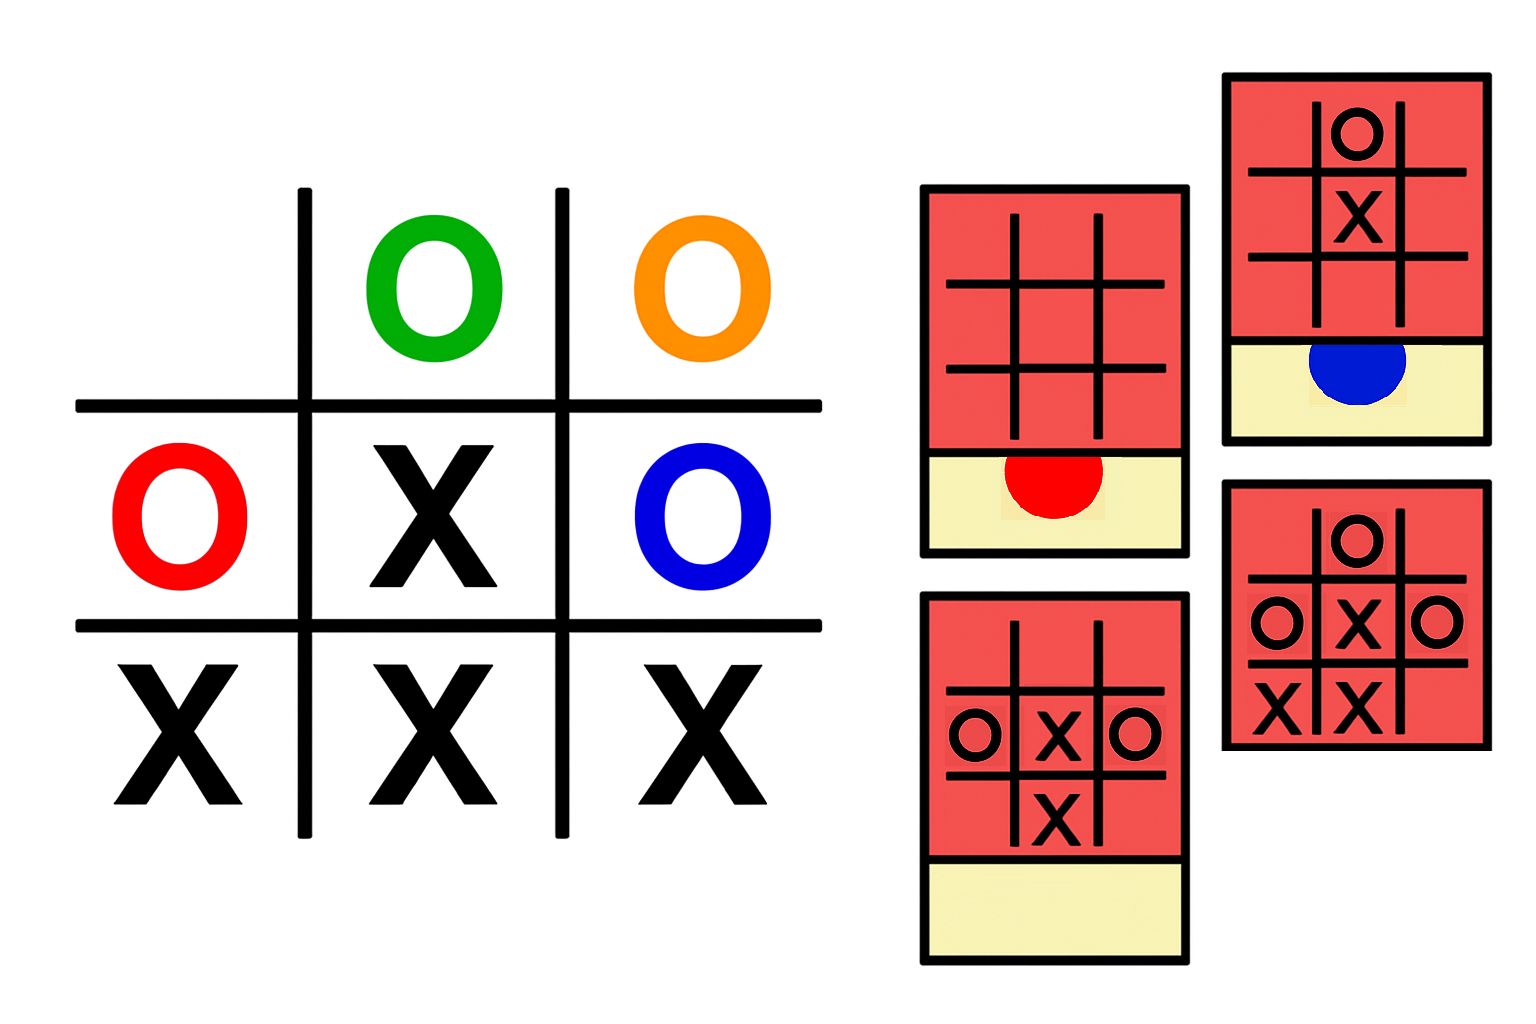
\includegraphics[width=.5\textwidth]{figures/menace_19.png}
\end{figure}
}
\only<20>{
\begin{figure}
    \centering
    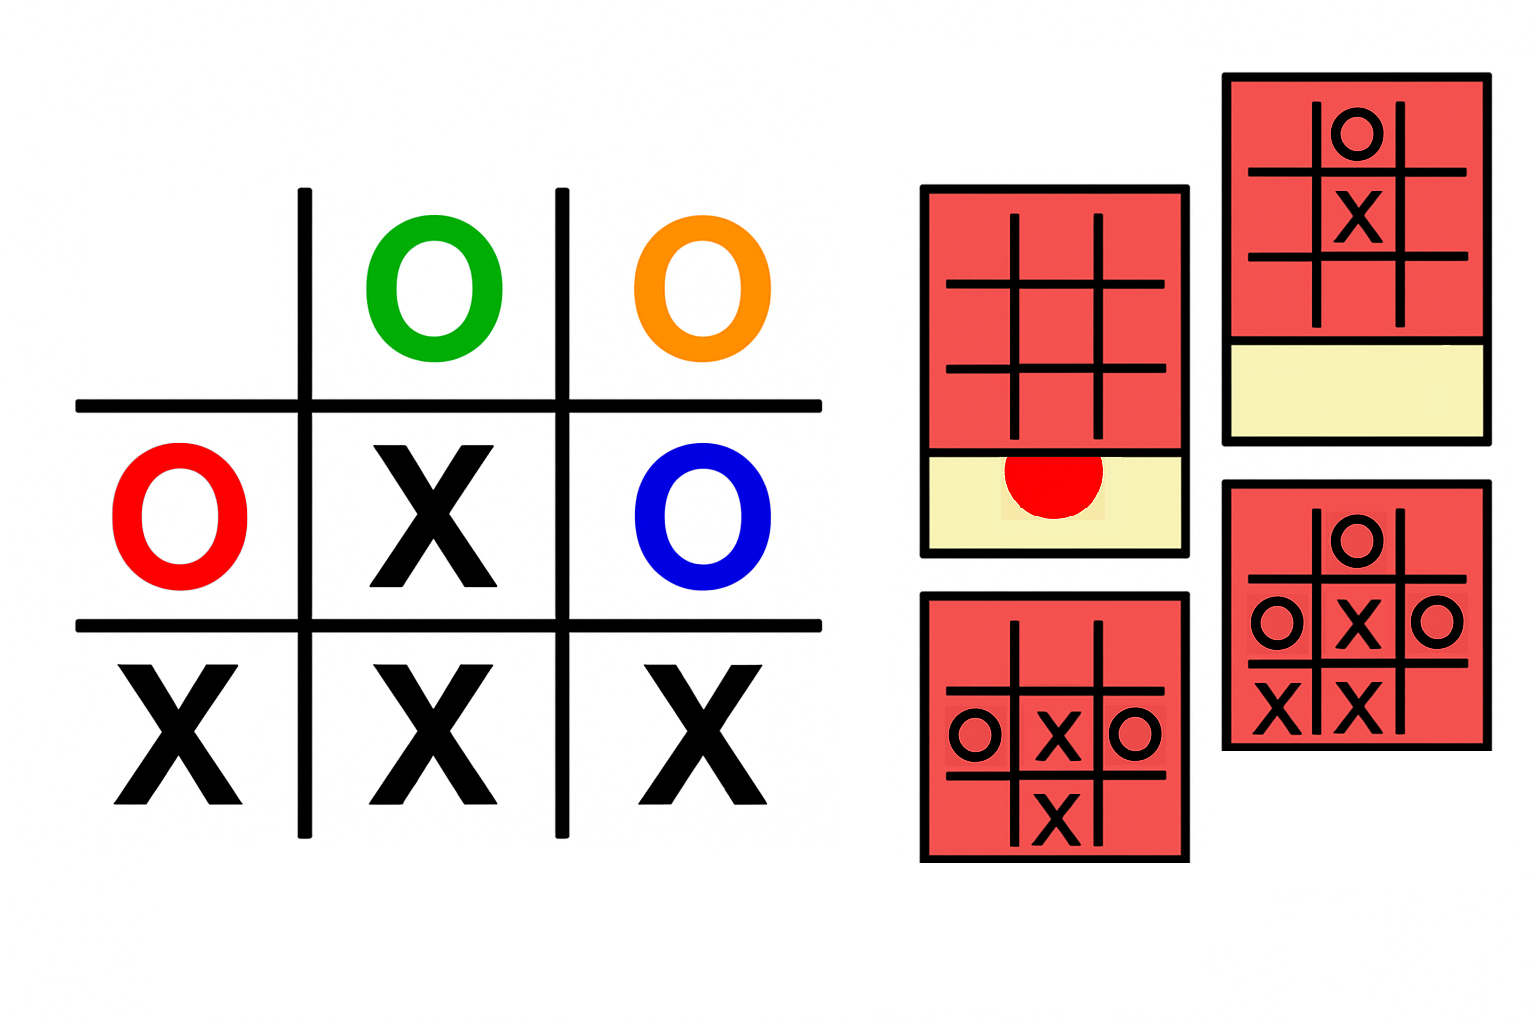
\includegraphics[width=.5\textwidth]{figures/menace_20.png}
\end{figure}
}
\only<21>{
\begin{figure}
    \centering
    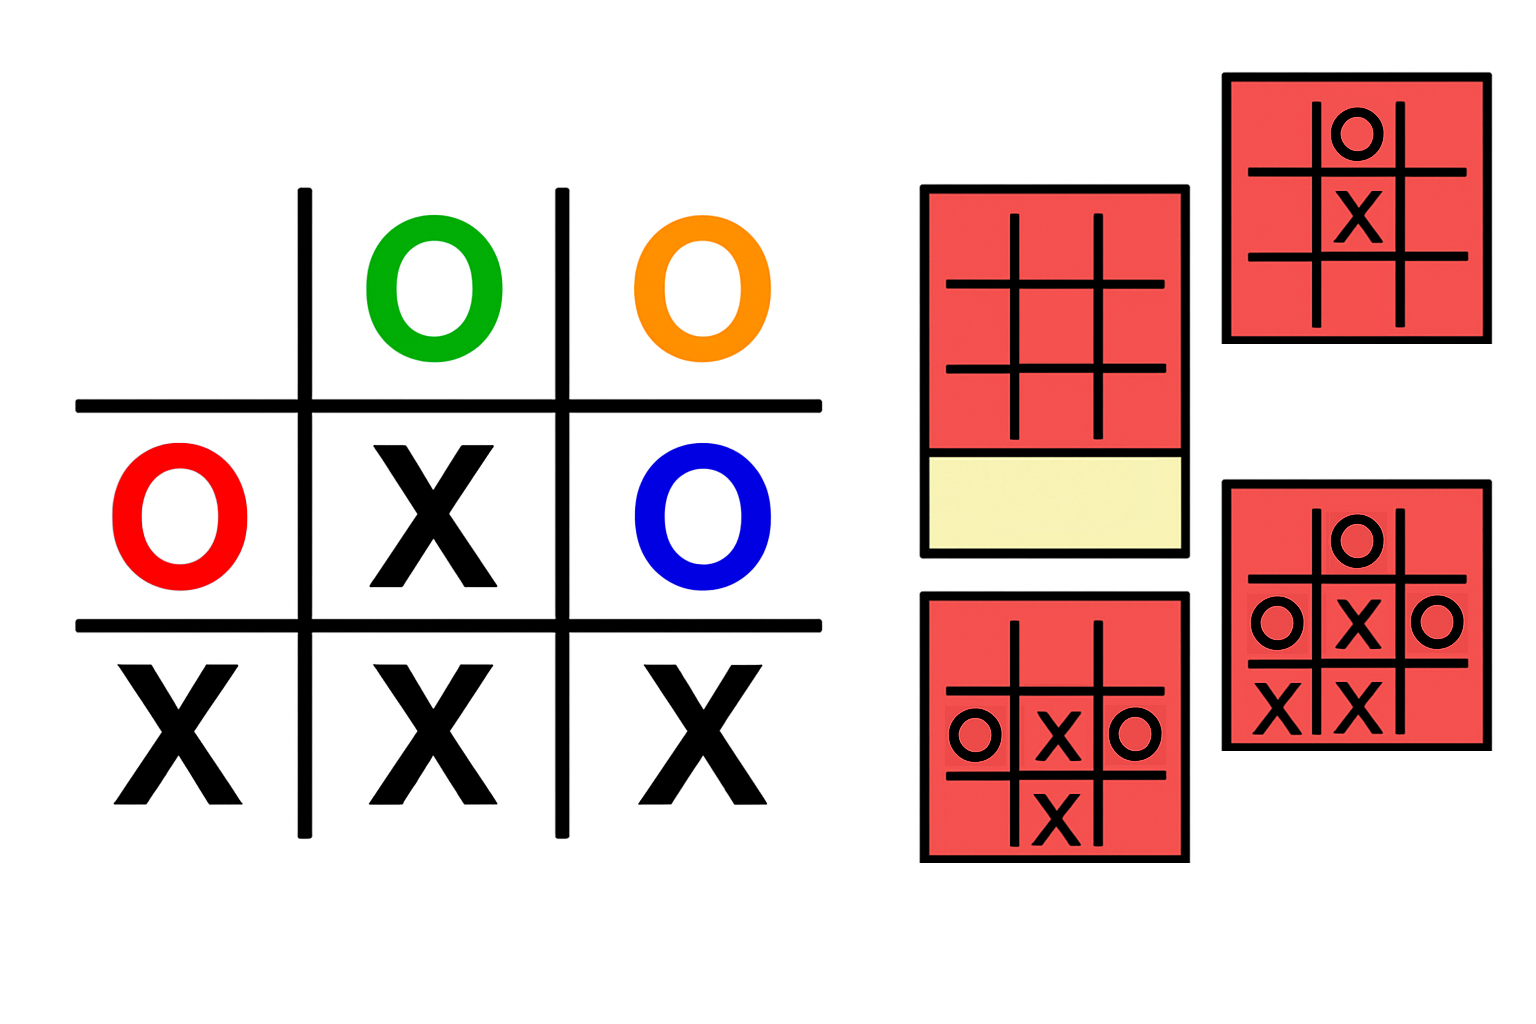
\includegraphics[width=.5\textwidth]{figures/menace_21.png}
\end{figure}
}
\only<22->{
\begin{figure}
    \centering
    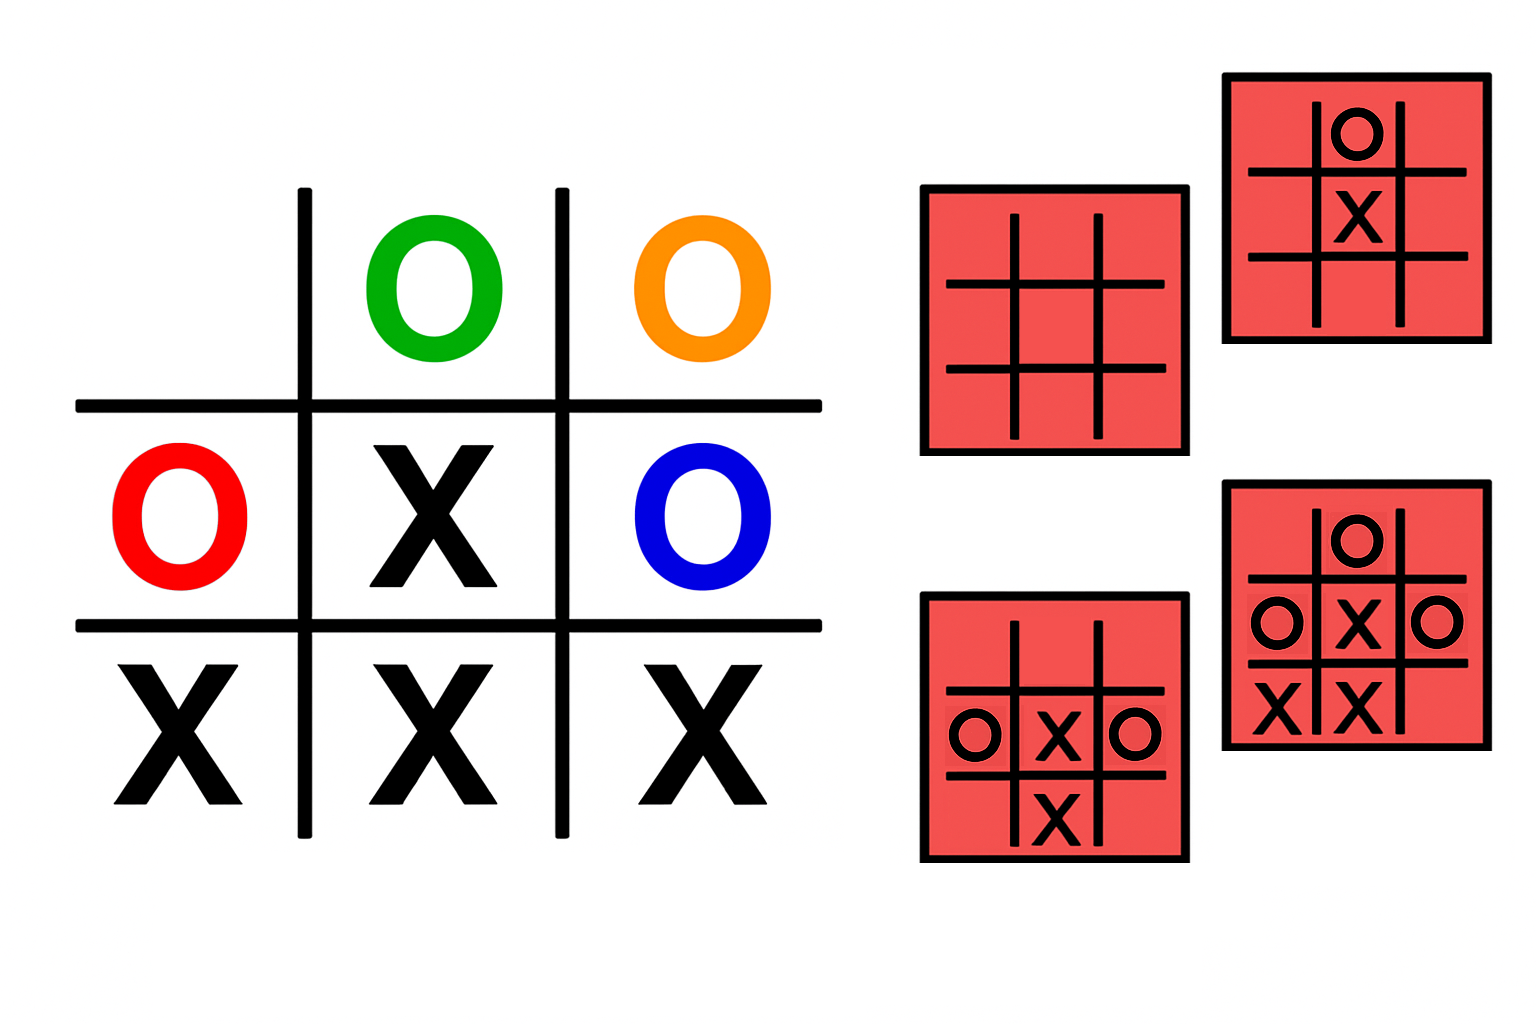
\includegraphics[width=.5\textwidth]{figures/menace_22.png}
\end{figure}
}

\medskip
\footnotesize\textit{Source: \href{https://www.mscroggs.co.uk/menace/}{Matthew Scroggs}}
\end{center}


\uncover<22>{
\begin{tabular}{llcll}
\textbf{Lose} & $\rightarrow$ & & Remove the bead from each box \\
\textbf{Win}  & $\rightarrow$ & & Add three beads to each box \\
\textbf{Draw} & $\rightarrow$ & & Add one bead to each box \\
\end{tabular}
}


\end{frame}


%
%
%\begin{frame}{Example: Inverted Pendulum}
%
%
%\begin{columns}[T]
%\begin{column}{0.6\textwidth}
%\begin{itemize}
   %\item State:
%
%$x(t),x'(t),\theta(t),\theta'(t)$
%
%\item Action: Force $F$
%\item Reward: 1 for any step  where pole balanced
%
%\end{itemize}
%\end{column}
%\begin{column}{0.4\textwidth}
%\scalebox{0.3}{
%\begin{tikzpicture}[line cap=round,line join=round,scale=2]
%
%\fill[draw=black,line width=1.5pt,line width=2pt,fill=BrewerBlue] (-6.4,-0.6) -- (-6.2,-0.6) -- (-6.2,-1.4) -- (-0.4,-1.4) -- (-0.4,-0.6) -- (-0.2,-0.6) -- (-0.2,-1.6) -- (-6.4,-1.6) -- cycle;
%\fill[draw=black,line width=1.5pt,line width=2pt,fill=BrewerBlue] (-4.6,-0.4) -- (-2.2,-0.4) -- (-2.2,-1.2) -- (-4.6,-1.2) -- cycle;
%\draw [line width=5.2pt] (-3.3,-0.38)-- (-1,2);
%\draw [draw=black,line width=1.5pt,line width=2pt,fill=BrewerBlue] (-3.9967614229502813,-1.1421149589850645) circle (0.25130295023545973cm);
%\draw [draw=black,line width=1.5pt,line width=2pt,fill=BrewerBlue] (-2.769226119268462,-1.151278199750565) circle (0.24609780622142172cm);
%
%
%%\draw (-1.3,-1) node {\huge \textbf{Environment}};
%%\draw (-1.5,2.8) node {\huge \textbf{Agent}};
%%\draw (-6,1) node {\Large \textbf{State}};
%%\draw (-2,1) node {\Large \textbf{Reward}};
%%\draw (1.5,1) node {\Large \textbf{Action}};
%\end{tikzpicture}
%}
%\end{column}
%\end{columns}
%
%\vspace{10mm}
    %Problem: Find $\pi:S\rightarrow A$ that  maximizes rewards
%
%\end{frame}

\begin{frame}{Important	Components in Reinforcement Learning}


Reinforcement learning agents may or may not include the following components:
\vspace{3mm}

\begin{itemize}
    \item \textcolor{red1}{\textbf{Model:}} $\mathbb{P}\left(s^{\prime} \mid s, a\right), \mathbb{P}(r \mid s, a)$
\begin{itemize}

\item  Environment dynamics and rewards
\end{itemize}
\item \textcolor{red1}{\textbf{Policy:}} $\pi(s)$

\begin{itemize} 
\item Agent action choices
\end{itemize}
\item \textcolor{red1}{\textbf{Value function:}} $V(s)$

\begin{itemize}
\item  Expected total rewards of the agent's policy 
\end{itemize}
\pause
\item \textcolor{red1}{\textbf{Quality function:}} $Q(s,a)$

\begin{itemize}
\item  Expected total rewards of taking a specific action in a given state %and then following a particular policy thereafter
\end{itemize}
\end{itemize}
    
\end{frame}


\begin{frame}{Bellman's Equation}
\begin{itemize}
    \item Optimal state value function $V^{*}(s)$

$$
V^{*}(s)=\max _{a} E[r \mid s, a]+\gamma \sum_{s^{\prime}} \mathbb{P}\left(s^{\prime} \mid s, a\right) V^{*}\left(s^{\prime}\right)
$$

\item Optimal state-action value function $Q^{*}(s, a)$

$$
\textcolor{red1}{Q^{*}(s, a)=E[r\mid s,a]+\gamma \sum_{s^{\prime}} \mathbb{P}\left(s^{\prime}\mid s,a\right) \max _{a^{\prime}} Q^{*}\left(s^{\prime}, a^{\prime}\right)}
$$

where $V^{*}(s)=\max _{a} Q^{*}(s, a)$\\
\quad\quad\quad $
\pi^{*}(s)=\underset{a}{\operatorname{argmax}} \; Q^{*}(s, a)
$ 
\end{itemize}    
\end{frame}



\section{Categorizing RL Agents}
{
\setbeamercolor{background canvas}{bg=BrewerBlue}
\begin{frame}
\centering
\Huge
\textcolor{white}{Categorizing RL Agents}
\thispagestyle{empty}
\end{frame}
}

\begin{frame}{Categorizing RL Agents}


  \begin{columns}[T]
\begin{column}{0.5\textwidth}
 \begin{tcolorbox}[colframe=black, boxrule=1pt, arc=6mm]
\textcolor{red1}{Value based}
\begin{itemize}
\item \textcolor{gray}{No policy (implicit)}
\item Value function

\end{itemize}
\textcolor{red1}{Policy based}
\begin{itemize}
    \item Policy
\item \textcolor{gray}{No value function}
 
\end{itemize}
\textcolor{red1}{Actor critic}
\begin{itemize}
    \item Policy
\item Value function
 
\end{itemize}

 \end{tcolorbox}
\end{column}
\begin{column}{0.5\textwidth}
\begin{tcolorbox}[colframe=black, boxrule=1pt, arc=6mm]

\textcolor{red1}{Model based}
\begin{itemize}
    \item Transition and  reward model

\end{itemize}
\textcolor{red1}{Model free}

\begin{itemize}
    \item \textcolor{gray}{No transition model (implicit)}
    \item \textcolor{gray}{No  reward model (implicit)}

\end{itemize}

\vspace{2.5cm}
\end{tcolorbox}
\end{column}
\end{columns}  
\end{frame}


\begin{frame}{Categorizing RL Agents}


  \begin{columns}[T]
\begin{column}{0.5\textwidth}
 \begin{tcolorbox}[colframe=black, boxrule=1pt, arc=6mm]
\textcolor{red1}{Value based}
\begin{itemize}
\item \textcolor{gray}{No policy (implicit)}
\item Value function

\end{itemize}
\textcolor{red1}{Policy based}
\begin{itemize}
    \item Policy
\item \textcolor{gray}{No value function}
 
\end{itemize}
\textcolor{red1}{Actor critic}
\begin{itemize}
    \item Policy
\item Value function
 
\end{itemize}

 \end{tcolorbox}
\end{column}
\begin{column}{0.5\textwidth}
\begin{tcolorbox}[colframe=black, boxrule=1pt, arc=6mm]

\textcolor{red1}{Model based}
\begin{itemize}
    \item Transition and  reward model

\end{itemize}
\textcolor{red1}{Model free}

\begin{itemize}
    \item \textcolor{gray}{No transition model (implicit)}
    \item \textcolor{gray}{No  reward model (implicit)}

\end{itemize}
\textcolor{red1}{Imitation Learning}

\begin{itemize}
    \item \textcolor{gray}{No transition model (implicit)}
    \item \textcolor{gray}{Reward model implicit through experts}

\end{itemize}

\end{tcolorbox}
\end{column}
\end{columns}  
\end{frame}



\begin{frame}{RL Algorithms}
\only<1>{
Dynamic Programming Backup
\begin{figure}
	\centering
		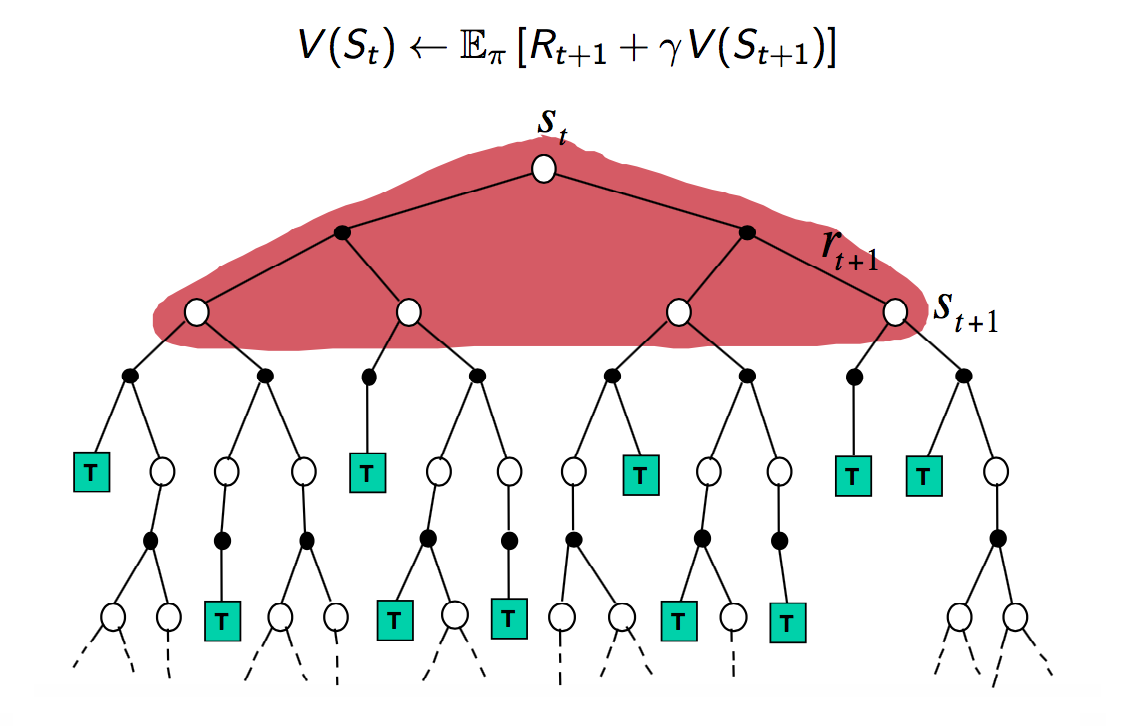
\includegraphics[width=0.60\textwidth]{figures/dynamic_programming_backup.png}
	\label{fig:DP}
\end{figure}
}
\only<2>{
Monte Carlo Backup
\begin{figure}
	\centering
		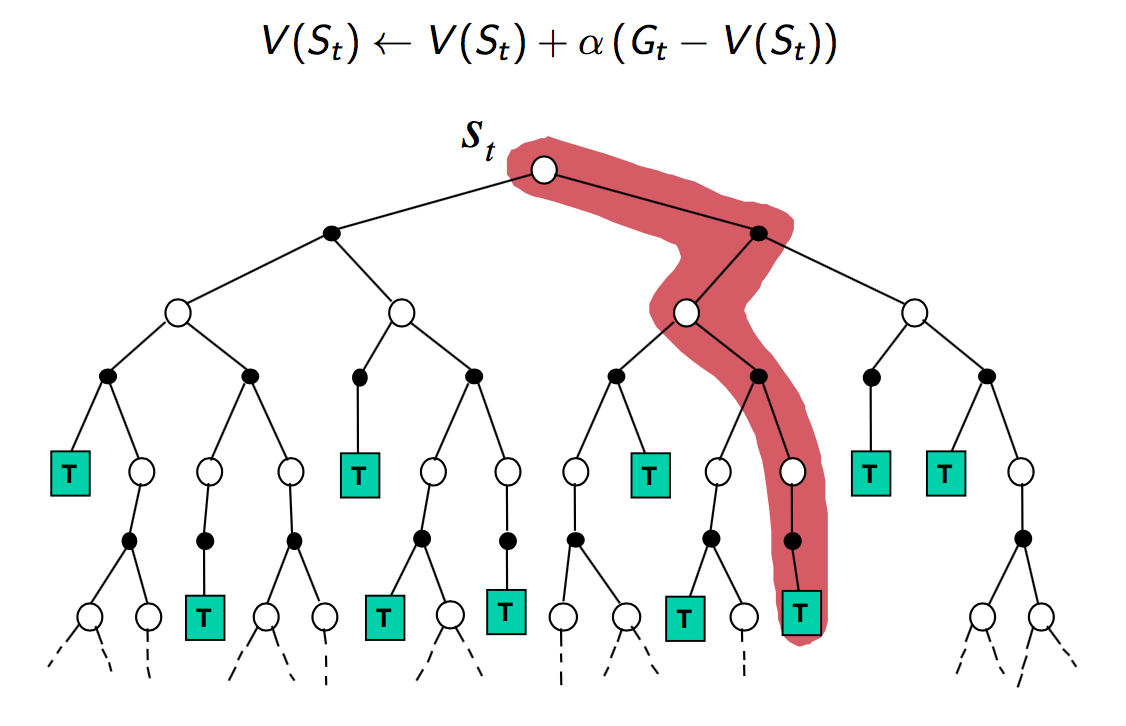
\includegraphics[width=0.60\textwidth]{figures/monte_carlo_backup.png}
	\label{fig:MC}
\end{figure}
}
\only<3>{
Temporal Difference Backup
\begin{figure}
	\centering
		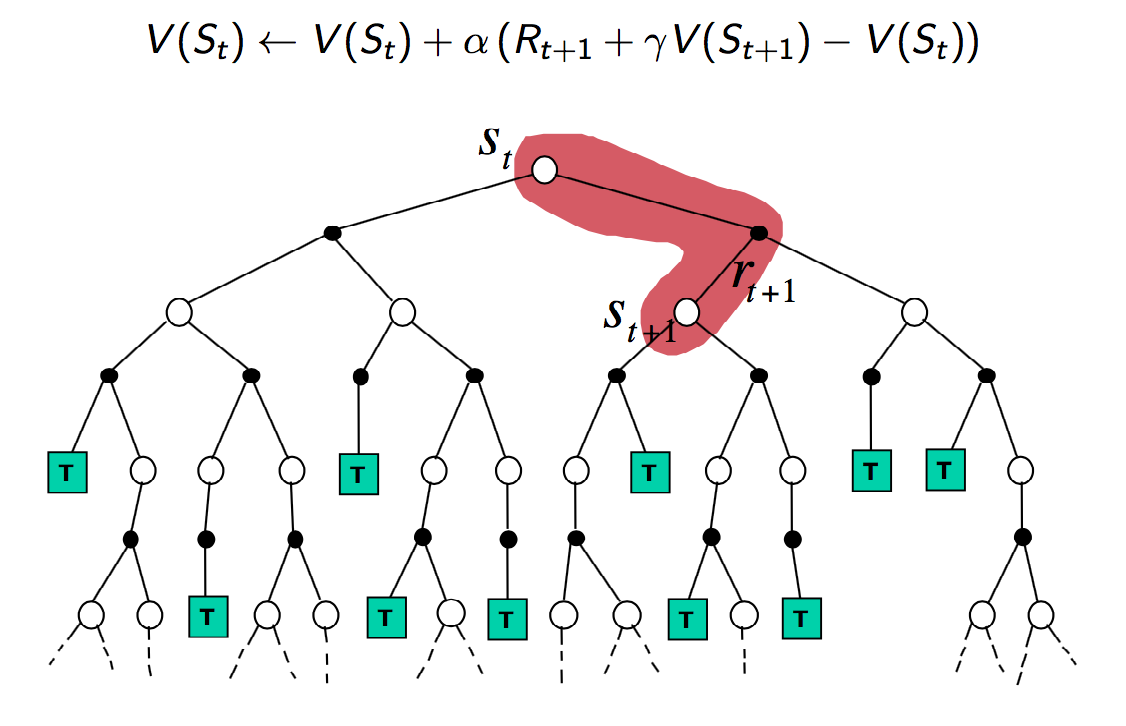
\includegraphics[width=0.60\textwidth]{figures/temporal_difference_backup.png}
	\label{fig:TD}
\end{figure}
}
\medskip
\hfill\footnotesize\textit{Source: David Silver}
\end{frame}







\begin{frame}{Toy Maze Example}


\begin{columns}[T]
\begin{column}{0.45\textwidth}
\centering
\scalebox{0.6}{

\begin{tikzpicture}[line cap=round,line join=round,x=0.75pt,y=0.75pt,yscale=-1,xscale=1]

%Shape: Rectangle [id:dp08468554766918346] 
\draw  [fill=BrewerBlue] (240.34,110.03) -- (300.07,110.03) -- (300.07,169.77) -- (240.34,169.77) -- cycle ;
\draw[line width=2pt]   (180.53,50) -- (420.11,50) -- (420.11,229.53) -- (180.53,229.53) -- cycle ;
%Straight Lines [id:da4224686848111512] 
\draw[line width=1.5pt]    (240.03,49.53) -- (239.53,229.03) ;
%Straight Lines [id:da6046918343336376] 
\draw[line width=1.5pt]    (300.03,49.53) -- (299.53,229.53) ;
%Straight Lines [id:da9626667234054846] 
\draw[line width=1.5pt]   (360.03,50.03) -- (359.53,229.53) ;
%Straight Lines [id:da267347571646644] 
\draw[line width=1.5pt]    (180.11,110) -- (419.53,110.53) ;
%Straight Lines [id:da6745979138164762] 
\draw[line width=1.5pt]    (180.03,169.53) -- (420.11,170) ;
%Shape: Square [id:dp1839161508205971] 

% Text Node
\draw (159.47,68) node [anchor=north west][inner sep=0.75pt]   [align=left] {{\Large $3$}};
% Text Node
\draw (159.47,130) node [anchor=north west][inner sep=0.75pt]   [align=left] {{\Large $2$}};
% Text Node
\draw (159.47,186) node [anchor=north west][inner sep=0.75pt]   [align=left] {\textbf{{\Large $1$}}};
% Text Node
\draw (201.47,234) node [anchor=north west][inner sep=0.75pt]   [align=left] {{\Large $1$}};
% Text Node
\draw (263.47,234) node [anchor=north west][inner sep=0.75pt]   [align=left] {{\Large $2$}};
% Text Node
\draw (325.47,234) node [anchor=north west][inner sep=0.75pt]   [align=left] {{\Large $3$}};
% Text Node
\draw (381.47,234) node [anchor=north west][inner sep=0.75pt]   [align=left] {{\Large $4$}};
% Text Node
\draw (202.47,70) node [anchor=north west][inner sep=0.75pt]  [font=\huge] [align=left] {{\textbf{r}}};
% Text Node
\draw (264.47,70) node [anchor=north west][inner sep=0.75pt]  [font=\huge] [align=left] {{\huge \textbf{r}}};
% Text Node
\draw (324.47,70) node [anchor=north west][inner sep=0.75pt]  [font=\huge] [align=left] {{\huge \textbf{r}}};
% Text Node
\draw (370.47,70) node [anchor=north west][inner sep=0.75pt]  [font=\huge] [align=left] {$\boldsymbol{+1}$};
% Text Node
\draw (202.47,131) node [anchor=north west][inner sep=0.75pt]  [font=\huge] [align=left] {\textbf{u}};
% Text Node
\draw (322,131) node [anchor=north west][inner sep=0.75pt]  [font=\huge] [align=left] {\textbf{u}};
% Text Node
\draw (370.47,131) node [anchor=north west][inner sep=0.75pt]  [font=\huge] [align=left] {$\boldsymbol{-1}$};
% Text Node
\draw (202.47,188) node [anchor=north west][inner sep=0.75pt]  [font=\huge] [align=left] {\textbf{u}};
% Text Node
\draw (260,186) node [anchor=north west][inner sep=0.75pt]  [font=\huge] [align=left] {\textbf{l}};
% Text Node
\draw (322,186) node [anchor=north west][inner sep=0.75pt]  [font=\huge] [align=left] {\textbf{l}};
% Text Node
\draw (383,186) node [anchor=north west][inner sep=0.75pt]  [font=\huge] [align=left] {\textbf{l}};
\end{tikzpicture}
}
\end{column}
\begin{column}{0.55\textwidth}
Start state: (1,1)\\
Terminal states: (4,2), (4,3)  
\\No discount: $\gamma$=1

\vspace{2mm}
Reward is -0.04 for  non-terminal states

\end{column}
\end{columns}

\vspace{6mm}
\centering
\begin{columns}
\begin{column}{0.4\textwidth}

Four actions:
\begin{itemize}
	\item up (\textbf{u}),
	\item left (\textbf{l}),
	\item right (\textbf{r}),
	\item down (\textbf{d})
\end{itemize}
\end{column}
\begin{column}{0.6\textwidth}
Do not know the transition probabilities

\vspace{3mm}
  \textcolor{red1}{What is the value $V(s)$ of being in state $s$}
\end{column}
\end{columns}
    
\end{frame}


\begin{frame}{Toy Maze Example (No Learning, Noise 20\%)}
\begin{figure}
	\centering
		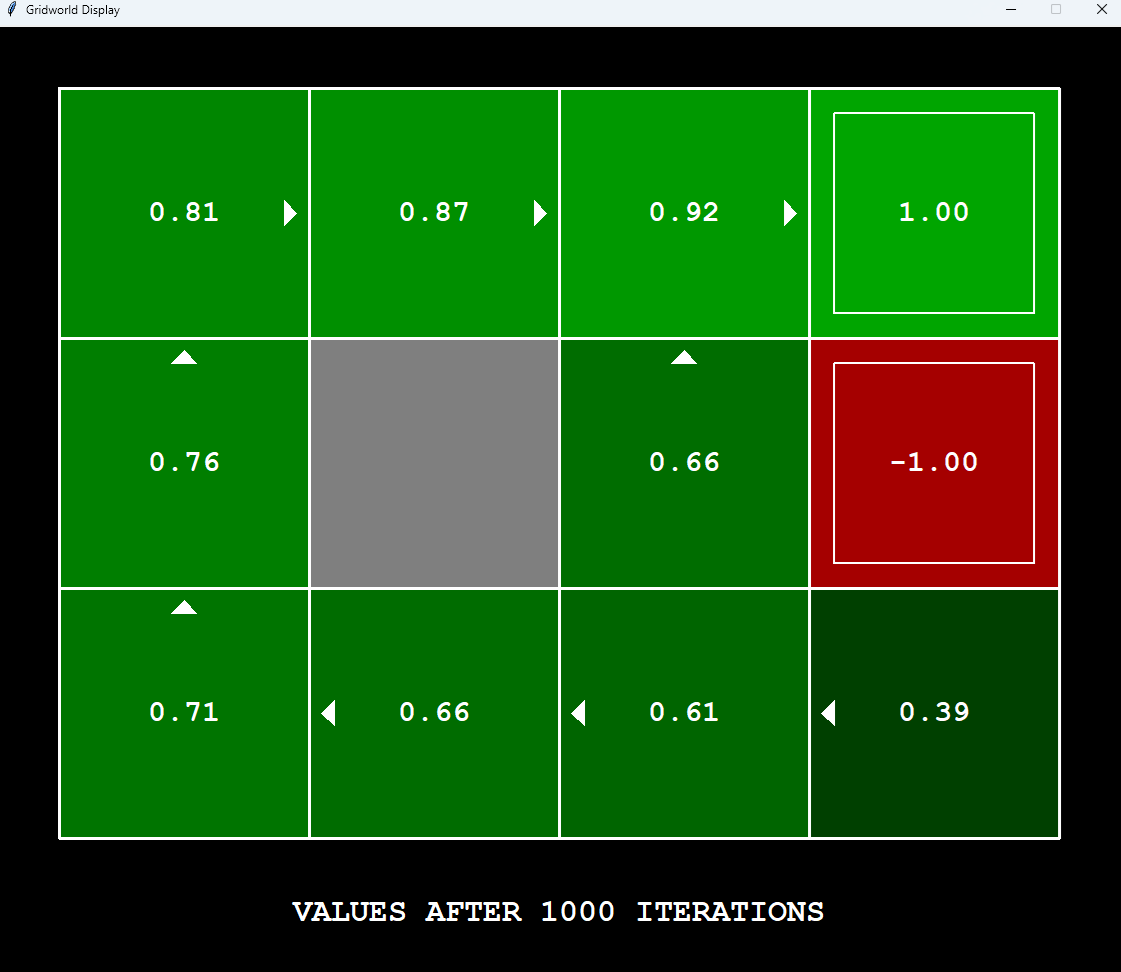
\includegraphics[width=0.80\textwidth]{figures/gridworld_values.png}
	\label{fig:gridworld_values}
\end{figure}

\end{frame}

\begin{frame}[t,allowframebreaks
]\nocite{*}
\frametitle{References}
\footnotesize
\bibliography{bib}
\end{frame}
\section{Takeaways}
{
\setbeamercolor{background canvas}{bg=BrewerBlue}
\begin{frame}
\centering
\Huge
\textcolor{white}{Takeaways}
\thispagestyle{empty}
\end{frame}
}



\begin{frame}{Takeaways}
\begin{itemize}
\item ``By three methods we may learn wisdom:
\begin{itemize}
	\item  First, by reflection, which is \sout{noblest} model-based RL;
	\item Second, by imitation, which is \sout{easiest} imitation learning; and
	\item third by experience, which is the \sout{bitterest} model free RL.''
\end{itemize}
\vspace{2em}
   \item RL agent types:
	 \begin{itemize}
		 \item value-based,
		 \item policy-based,
		 \item value-policy-based (actor-critic),
		 \item model-based,
	   \item model-free
	   \item imitation learning
	 \end{itemize}

\end{itemize}
\end{frame}




\end{document}
